\documentclass[11pt]{article}
\usepackage[T1]{fontenc}
\usepackage{lmodern}
\usepackage[margin=1.05in]{geometry}
\usepackage{amsmath,amssymb,amsthm,mathtools}
\usepackage{microtype}
\usepackage{enumitem}
\usepackage{needspace}
\usepackage{float}
\usepackage{tikz}
\usetikzlibrary{arrows.meta,positioning,calc}
\usepackage[hidelinks]{hyperref}
\usepackage{bookmark}
\newtheorem{theorem}{Theorem}[section]
\newtheorem{proposition}[theorem]{Proposition}
\newtheorem{lemma}[theorem]{Lemma}
\newtheorem{corollary}[theorem]{Corollary}
\theoremstyle{definition}
\newtheorem{definition}[theorem]{Definition}
\newtheorem{convention}[theorem]{Convention}
\theoremstyle{remark}
\newtheorem{remark}[theorem]{Remark}
\newcommand{\Z}{\mathbb Z}
\newcommand{\R}{\mathbb R}
\newcommand{\Q}{\mathbb Q}
\newcommand{\PD}{\mathrm{PD}}
\newcommand{\CAT}{\operatorname{CAT}}
\DeclareMathOperator{\Wh}{Wh}
\DeclareMathOperator{\im}{im}
\DeclareMathOperator{\coker}{coker}
\DeclareMathOperator{\rank}{rank}
\setlist[enumerate]{itemsep=3pt,topsep=5pt}
\setlist[itemize]{itemsep=3pt,topsep=5pt}
\emergencystretch=2em
\clubpenalty=10000
\widowpenalty=10000
\hypersetup{pdftitle={A PD4 group without an aspherical manifold model},pdfauthor={OpenAI}}
\title{A PD4 group without an aspherical manifold model}
\author{OpenAI}
\date{September 24, 2026}
\begin{document}
\maketitle
\begin{abstract}
We construct a finitely presented integral Poincar\'e duality group of
dimension four that has a finite classifying space but is not the fundamental
group of any closed aspherical topological four-manifold. This gives a negative
answer to Wall's manifold-realization question in dimension four.
\end{abstract}

\section{Introduction}\label{sec:introduction}

A closed aspherical manifold is determined up to homotopy by its
fundamental group. Poincar\'e duality therefore supplies a necessary
algebraic condition on that group. The manifold-realization question asks
whether this condition, together with the appropriate finiteness
assumptions, is sufficient. Here the category matters: a finite Poincar\'e
complex, a homology manifold, and a smooth manifold are different possible
realizations. We address closed \emph{topological} manifolds in the same
dimension as the duality group.

An oriented integral Poincar\'e duality group $G$ of dimension $n$, or
\emph{oriented integral $\PD_n$ group}, has a finite resolution of the
trivial $\Z G$-module $\Z$ by finitely generated projective modules;
its cohomology with coefficients in $\Z G$ vanishes outside degree $n$
and is $\Z$ in degree $n$, with trivial right $G$-action. A finite
classifying space is a finite CW complex with fundamental group $G$
and contractible universal cover. Such a space provides a finite free
resolution, but its existence alone does not provide a manifold model.

Wall asked whether every integral Poincar\'e duality group is the
fundamental group of a closed aspherical manifold
\cite[Problem~G2]{WallProblems}. The finiteness condition requires care.
Davis used reflection groups to turn the finiteness examples of
Bestvina and Brady into integral $\PD_n$ groups that are not finitely
presented, for every $n\geq4$ \cite[Theorem~C]{DavisCohomology}.
Since a closed manifold has finitely presented fundamental group,
these examples answer the unqualified question. The remaining
manifold-realization question asks the same thing for \emph{finitely
presented} integral Poincar\'e duality groups; it is Question~3.4 in
Davis's survey~\cite{DavisPD} and Conjecture~7.29 in the cited version
of L\"uck's survey~\cite{LuckFJ}. Kielak's 2026 survey records that
no counterexamples to this formulation were known
\cite[Section~4.1]{Kielak}.

The coefficient ring is equally important. Fowler constructed
torsion-free finitely presented rational Poincar\'e duality groups that
cannot be realized by closed aspherical ANR rational homology
manifolds~\cite[Theorem~2.1]{Fowler}. His examples have no finite
classifying space. The example below instead satisfies integral
duality and already has a finite four-dimensional classifying space;
its obstruction concerns the passage from that Poincar\'e complex to a
closed topological manifold.

\begin{theorem}\label{thm:main}
There is a finitely presented group $G$ with a finite, oriented,
four-dimensional aspherical Poincar\'e complex $Q$ such that
\[
 H^i(G;\Z G)=0\quad(i\ne4),\qquad H^4(G;\Z G)\cong\Z
\]
with trivial right $G$-action on the last group, but no closed aspherical
topological four-manifold has fundamental group $G$.
In particular the trivial left $\Z G$-module $\Z$ has a finite resolution
by finitely generated free modules.
\end{theorem}

Theorem~\ref{thm:main} refutes the assertion quantified simultaneously
over all dimensions $n\geq3$, without asserting a counterexample in every
dimension. The orientation qualification causes no additional issue:
the orientation character of any hypothetical aspherical manifold with
group $G$ would equal the right action on its dualizing module and hence
would be trivial.

\subsection{The source of the obstruction}
Our starting point is the marked geometric and tensor obstruction in
\emph{A marked tensor obstruction to four-dimensional disk
embedding}~\cite{TO}. Its geometric package records a finite family of
based loop relations, including independently chosen conjugating paths,
together with algebraic dual spheres. Its algebraic package turns a
compatible cut configuration into potentials and exact identities over
a ring with nilpotent parameters. A finite tensor theorem excludes those
identities. Section~\ref{ch:inputs} recalls the complete interface,
including the mixed nilpotent terms and the memberships in actual
gradient ideals. The marked geometry, algebraicity, formal comparison,
and finite tensor theorem are inputs from the companion; the transfer
to arbitrary marked topological fillings is proved here.

The argument has two principal geometric ingredients beyond that input.
First, we construct a smooth chamber $D$ with boundary $S$ and a specified
hyperbolic basis for its entire middle homology. Attaching three-cells along that basis
gives a marked graph-type Poincar\'e pair $(P,S)$, but its marked boundary
admits no topological graph-type filling.
Here $H=\pi_1D$ is free and $BH$ denotes a finite graph with fundamental
group $H$; the space $P$ is homotopy equivalent to $BH$.
The marking is a specified map $S\to BH$. A
\emph{marked graph-type filling} is a compact topological four-manifold
with identified boundary $S$ and a homotopy equivalence to $BH$ extending
that map up to homotopy. This requirement retains information about the
boundary loops throughout the construction.
The extension of the cut obstruction to topological fillings uses
smoothing off isolated points and a differential-form complex that
computes the cohomology \emph{with those points filled}. Second, we show
that a hypothetical manifold model for a reflection of $P$ would produce
exactly such a forbidden filling. This requires a stable product with a
specified sphere marking, followed by a destabilization argument. An
unmarked stable homeomorphism would not suffice.

The chamber obstruction is a relative manifold-realization statement:
the manifold must realize the homotopy type of the given Poincar\'e pair
relative to its identified boundary. Davis and Hillman prove such relative realization for an
aspherical Poincar\'e pair with nonempty closed manifold boundary in
dimensions at least five, assuming the $K$- and $L$-theoretic
Farrell--Jones conjectures, and in dimension four for elementary
amenable fundamental groups~\cite[Theorem~D]{DavisHillman}. Our chamber
has nonabelian free fundamental group, and its marked filling obstruction concerns
the four-dimensional case outside that elementary amenable hypothesis.
Reflection converts this relative obstruction into the closed
manifold-realization question of Theorem~\ref{thm:main}.

\subsection{Proof architecture}
The reflection method developed by Davis~\cite[Sections~13 and~15]{Davis1983}
provides the framework for closing the chamber. Our construction closes
the pair to an aspherical Poincar\'e
complex $Q$ and reflects $D$ to a closed manifold $N\to Q$. A
support-tree construction gives the relevant right-angled Coxeter
extension of the free chamber group a proper cocompact CAT(0) model.
This auxiliary model supplies assembly information; the chamber
development retains the four-dimensional topology and its sphere classes.
The CAT(0) action places $G=\pi_1Q$ among the groups to which the Farrell--Jones
theorems apply~\cite{BL,Wegner}. If $Q$ had a manifold model $M$, the
four-dimensional surgery result of Kasprowski--Land~\cite{KL}, followed
by a stable product theorem, would make all the prescribed hyperbolic
pairs of a stabilization of $N$ geometrically standard.

Lift these finite marked data to the reflection development. In a large
finite union of chambers, cap every boundary summand except the central
one. Remove standard pairs labelled by a large inner ball. The remaining
sphere problems are far from the central chamber, where radial directions
in the Davis complex make every bounded local construction small.
Grope separation follows Freedman--Quinn's finite-cover strategy
\cite[Section~2.10.2]{FQ} and groups the upper branches over finitely many
contractible direction patches. The essential requirement is that an
entire resulting loop system stays over one such patch, even when it
passes through many intersections. This replaces precisely the goodness-dependent
null-loop step of Powell--Ray--Teichner~\cite{PRT}, and not their theorem's
group hypothesis by fiat. The subsequent disk construction is
uncontrolled and may range through the whole compact manifold. Surgery
then gives the forbidden filling of $S$.

Section~\ref{ch:section} constructs the marked chamber and proves its
filling obstruction. Section~\ref{rf:section} reflects it to obtain
$Q$, verifies integral duality, and supplies the two geometric models
used later. Section~\ref{st:setup} uses a hypothetical manifold model to
realize every prescribed sphere pair after stabilization.
Section~\ref{ct:section} caps a finite chamber union, removes the inner
standard pairs, and uses direction control to remove the remaining
middle homology. Its output is the marked filling excluded by
Section~\ref{ch:section}.

\begin{figure}[H]
\centering
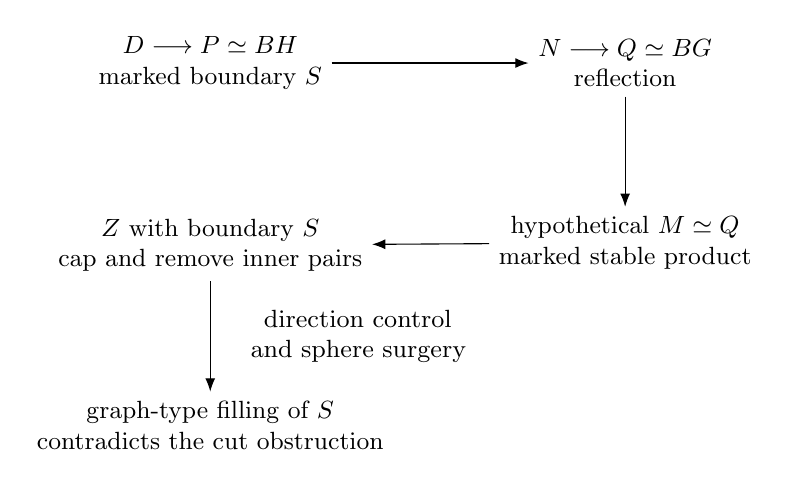
\begin{tikzpicture}[>=Latex, node distance=14mm and 25mm,
  every node/.style={align=center,font=\small}]
\node (D) {$D\longrightarrow P\simeq BH$\\marked boundary $S$};
\node[right=of D] (N) {$N\longrightarrow Q\simeq BG$\\reflection};
\node[below=of N] (M) {hypothetical $M\simeq Q$\\marked stable product};
\node[below=of D] (Z) {$Z$ with boundary $S$\\cap and remove inner pairs};
\node[below=of Z] (W) {graph-type filling of $S$\\contradicts the cut obstruction};
\draw[->] (D) -- (N);
\draw[->] (N) -- (M);
\draw[->] (M) -- (Z);
\draw[->] (Z) -- node[right,text width=35mm] {direction control\\and sphere surgery} (W);
\end{tikzpicture}
\caption{The two uses of the chamber. Its middle spheres permit the
reflection and stable-surgery construction; its marked boundary forbids
the filling obtained at the end.}
\label{fig:architecture}
\end{figure}

\subsection{Conventions}
All manifolds in the surgery argument are oriented and all unqualified
homology groups have integral coefficients. For a connected space with
fundamental group $\Gamma$, regular coefficients $\Z\Gamma$ mean the
homology of its universal cover. We fix lifts and paths to a basepoint
when recording sphere classes. The involution on an oriented group ring
is $\overline{\sum n_g g}=\sum n_g g^{-1}$.
A hyperbolic plane over $\Z\Gamma$ has matrix
$\left(\begin{smallmatrix}0&1\\1&0\end{smallmatrix}\right)$.
For immersed sphere representatives, the phrase \emph{framed hyperbolic
system} also includes vanishing Wall self-intersection obstructions.

All stabilizations are interior connected sums with $S^2\times S^2$ and
leave boundary markings unchanged. Specific references to
Freedman--Quinn~\cite{FQ} use the January 2013 reformatted edition's
numbering.

\section{A chamber with no marked graph filling}
\label{ch:section}

The obstruction will first be placed in a compact chamber.  Its boundary
marking is essential: the obstruction does not merely assert that some
disk problem has no solution.

\begin{proposition}[The marked chamber]
\label{ch:chamber}
There are a compact connected oriented smooth four-manifold $D$, its
connected boundary $S$, a finitely generated free group $H$, and a map
$c:D\to BH$ with the following properties.
\begin{enumerate}
\item The map $c$ induces an isomorphism on fundamental groups, and $D$
has the homotopy type of a finite graph with $2k$ two-spheres attached
at its basepoint.  Its module $\pi_2D$ has a specified hyperbolic basis
over $\Z H$, represented by framed immersed spheres with vanishing
quadratic self-intersection obstructions.
\item Attach a three-cell to each basis sphere, and denote the resulting
space by $P$.  Then $(P,S)$ is an oriented Poincar\'e pair of formal
dimension four, and $P\simeq BH$.  The boundary marking is
$c|_S:S\to BH$.
\item There is no compact oriented topological four-manifold $D'$ with
boundary identified with $S$ and a homotopy equivalence $c':D'\to BH$
whose restriction to $S$ is homotopic to $c|_S$.
\end{enumerate}
\end{proposition}

Here and below, sphere classes and intersections use fixed whiskers and
deck translations.  A hyperbolic pair has zero squares, mutual product
$1$, and zero framing and Wall self-intersection obstructions.  We prove
the proposition without using an embedded surgery on $D$.

\subsection{The geometric and tensor inputs}
\label{ch:inputs}

We use the marked geometric construction of \cite[Section~2]{TO}, rather
than only its main disk-nonembedding theorem. The marked bodies and
exterior duals are supplied by its Lemmas~2.3 and~2.4. Its
Proposition~2.2 and Lemmas~2.5--2.6 give the cut consequences under
hypothetical disk replacements; those conditional conclusions are
distinct from the marked geometric construction itself.
We recall the precise data needed here.
Fix $m\geq5$ and $p\geq9$.  Start with a four-dimensional one-handlebody
on $2m+p$ handles, attach cancelling two-handles to the first $2m$
handles with product framings, and plumb these two-handles in $m$ pairs,
interchanging the two coordinate directions at every plumbing.
The resulting smooth oriented manifold $X$ has graph homotopy type.
Its cover associated to the plumbing quotient $\pi_1X\to F_m$ is a
tree of blocks, each a one-handlebody on $p$ extra generators; neighboring
blocks meet in a product four-ball.  The exposed boundary of a block is
\[
 K_v=\#^p(S^1\times S^2)\setminus
       \operatorname{int}\nu(L_{2m}),
\]
where $L_{2m}$ is an unlink in a ball.  Its port meridians
$x_1,\ldots,x_{2m}$ and extra loops $l_1,\ldots,l_p$ form a free basis.
At each join the meridian on one side is the longitude on the other.

Write $\mathcal C=\{1,l_1,\ldots,l_p\}$.  The marked-body construction
installs a disjoint two-stage grope body for every ordered triple of
distinct ports and every independent choice
\[
 X_a=c_a x_{r_a}^{\delta_a}c_a^{-1},\qquad
 c_a\in\mathcal C,\quad \delta_a\in\{1,-1\},\quad a=1,2,3.
\]
Its lower surface is a punctured torus: one branch has a single cap,
and the other carries the upper punctured torus with its two caps.
All tip tracks, conjugating paths, and product framings are specified.
The initial boundary word $R$ satisfies
\begin{equation}
\label{ch:laws}
 R|_{X_a=1}=1\quad(a=1,2,3),\qquad
 R\equiv[X_1,[X_2,X_3]]\pmod{\Gamma_4F(X_1,X_2,X_3)}.
\end{equation}
Internal changes of the marked paths are allowed by these identities;
one must retain the entire finite family, not replace it by one
unconjugated commutator.

Let $F_1,\ldots,F_k$ be the lower punctured tori, with symplectic bases
$(a_j,b_j)$, where $a_j$ is the single-cap branch.  Delete their open
product tubes, including the proper edge collars, to obtain $E$.
Lemma~2.4 (Algebraic duals in the exterior) of \cite{TO} supplies
the truncated single caps $f_j$ and framed spheres $g_j$ in $E$ such
that
\begin{equation}
\label{ch:exterior-duals}
 \lambda(f_i,g_j)=\delta_{ij},\qquad
 \lambda(g_i,g_j)=0,\qquad \widetilde\mu(g_j)=0
 \quad\text{over }\Z[\pi_1E].
\end{equation}
The framing on $f_j$ is the surface-compression framing.  The $g_j$
are compressed normal-circle tori over the $b_j$ curves; their
individual representatives have trivial normal bundle.  Equation
\eqref{ch:exterior-duals} is a group-ring statement before any
meridians are killed.

We also recall exactly how the cut obstruction is used.  Suppose that a
compact smooth oriented four-manifold with the marked graph type of
the parity cover of $X$ has two connected vertex pieces $A,B$, with
outside faces $K_A,K_B$, and $2m$ connected three-dimensional cuts
$Y_i$, each with its prescribed coordinate torus as its entire boundary.
Orient $Y_i$ as a face of $A$, so its orientation as a face of $B$
is opposite.
Suppose the differences of restrictions give an isomorphism in degree
two and, in degree one, an isomorphism after the extra-loop evaluations
are set to zero.  Suppose further that precisely $m$ joins are active:
at an active join the surviving coordinate meridian is at $A$, whereas
the other coordinate is the meridian at $B$.  Require every marked law
\eqref{ch:laws} in its respective vertex group, and the free ambient
background in which the port meridians are trivial and the named extra
letters can be assigned independently.

These data cannot exist.  Indeed, Proposition~6.1 (Vertex data) of
\cite{TO} gives a characteristic-zero field $K$ (one may take
$\mathbb C((\sigma))$), separate coordinate blocks $h_i$ of total
dimension $N$, and algebraic power-series germs $F_i(h_i)$ and
$b_i(h_i)$, with $b_i$ indexed by the active set $I$, $|I|=m$.
The germs are normalized by $F_i(0)=b_i(0)=0$.  Set
\begin{equation}
\label{ch:tensor-ring}
 T=K[t_i:i\in I]/(t_i^2:i\in I),\qquad
 S_0=\sum_iF_i,\qquad S_t=S_0+\sum_{i\in I}t_i b_i.
\end{equation}
There are formal parametrizations
\[
 H_L(x,t)\in(x,t)T[[x]]^N,\qquad
 H_R(y)\in(y)K[[y]]^N,
\]
where $x$ has $d$ coordinates and $y$ has $N-d$ coordinates.  Their
central tangent maps $\partial_xH_L(0,0)$ and $\partial_yH_R(0)$
are injective with complementary images in $K^N$; nilpotent constant
displacements of $H_L$ are allowed.  They satisfy
\begin{equation}
\label{ch:tensor-vanishing}
 S_t(H_L)=0,\qquad S_0(H_R)=0.
\end{equation}
For every three distinct active indices $i,j,k$, they satisfy
\begin{align}
 t_it_jt_k&\in
 \bigl((\partial_{h_\nu}S_t)(H_L):\nu=1,\ldots,N\bigr)
                  \subset T[[x]],\label{ch:tensor-left}\\
 (b_ib_jb_k)(H_R)&\in
 \bigl((\partial_{h_\nu}S_0)(H_R):\nu=1,\ldots,N\bigr)
                  \subset K[[y]].\label{ch:tensor-right}
\end{align}
Theorem~3.1 (Finite tensor obstruction) of \cite{TO} rules out
\eqref{ch:tensor-ring}--\eqref{ch:tensor-right} for $m\geq5$.
In particular, the memberships are in the actual gradient ideals,
not their radicals, and $T$ retains all mixed square-free monomials.
The independent conjugators in the full law list are what supply all
these triple identities. These two source results, together with the
marked edge potentials, algebraicity and formal comparison of
\cite[Proposition~4.5, Theorem~5.1 and Proposition~5.2]{TO}, are the
tensor obstruction used here.

\subsection{The exterior with its side marking}
\label{ch:exterior}

The imported geometry supplies the surfaces and their algebraic duals.
We now use those data to construct $D$, keeping track of the actual
tube-side maps. This marking will identify the boundary of a hypothetical
filling with the loop data needed for the tensor contradiction.

We make one placement refinement of the marked-body construction.
Place its longitudinal tip annuli on disjoint parallels outside
sufficiently thin attaching solid tori in the initial one-handlebody
boundary, and put the finitely many connectors in their complement.
This is possible by the marked handlebody model: the bodies are boundary
joins of the separated annular collars.  The complement of the attaching
solid tori survives in the boundary after the two-handles are attached;
the plumbing ports are on the new belt-handle portions.  Thus the
unpushed lower surfaces lie in the final exposed boundary of $X$.
The independent ribbon twists matching the cap framings are made in
the separated parallel tubes.  They do not pass a body across a
plumbing join.  The returning tip collars alone are lengthened back
to product parallels on the attaching regions and then into the cores.
The construction and intersection calculation of
\eqref{ch:exterior-duals} are unchanged.

Consequently the $F_j$ are proper inward pushes of disjoint boundary
surfaces, with returning collars at their initial boundary curves.
Moreover $F_j\to X$ is null-homotopic.  The three tip loops bound the
corresponding core caps in $X$; hence the bottom $a_j$ and $b_j$ loops
die in $\pi_1X$.  Since $X$ has graph homotopy type and $F_j$ retracts
to a graph, this proves the assertion about the whole surface map.

\begin{lemma}[The marked exterior model]
\label{ch:exterior-model}
With the surface-product trivializations, the exterior and its tube-side
maps have the homotopy-pushout model
\[
 E\simeq X\cup_{\coprod_jF_j}\coprod_j(F_j\times S^1),
\]
where each gluing map to $F_j\times S^1$ is the inward section.
The displayed $F_j\times S^1$ maps represent the actual tube sides.
\end{lemma}

\begin{proof}
It is enough to describe one surface; the constructions have disjoint
collars.  Write $B=\partial X$ and $K=\partial F$.  Before rounding
corners, put the pushed surface at a horizontal collar level, with
vertical walls along $K$ returning to the boundary.  The inner part of
the exterior has homotopy type $X$, the outer part has homotopy type
$B\setminus K$, and their overlap has homotopy type $B\setminus F$.
Product slices, thickened by a variable positive width off the deleted
surface, give this homotopy-pushout decomposition.

In $B\setminus K$, take a two-sided neighborhood of
$F^\circ=F\setminus K$ whose width decreases to zero near $K$.
Relative to $B\setminus F$, it is a bridge over $F^\circ$, joining
the two sides of the cut.  Replace $F^\circ$ in this diagram by a
slightly shrunken copy $F_0$; this is an objectwise homotopy equivalence.
The actual deleted surface and $K$ are unchanged.  In the rectangular
normal coordinates to its horizontal copy, split the tube circle over
$F_0$ into its outer and inward semicircles.  The outer semicircle is
the bridge.  The inward semicircle lies in the inner $X$ piece and
gives a specified homotopy between the bridge's endpoint maps.

Using that homotopy to identify the endpoints replaces the bridge by
$F_0\times S^1$, attached along its inward section.  Its circle is
precisely the outer bridge followed by the inward return, hence the
actual normal circuit.  Finally $F_0\to F$ and
$F_0\times S^1\to F\times S^1$ are homotopy equivalences.  This
also accounts for the proper edge collars and proves the assertion
about the side maps, not just the absolute homotopy type of $E$.
\end{proof}

For each $j$, regard a solid torus $V_j$ as a compression body from
the punctured torus $F_j$ to a disk, compressing $a_j$.  Define
\[
 D=E\cup_{\coprod_j(F_j\times S^1)}
                  \coprod_j(V_j\times S^1).
\]
All gluings use the just specified product framings; round corners.
The remaining disk face of $\partial V_j$ contributes a solid torus
to the new boundary.  Hence $S=\partial D$ is the surface-framed
surgery of $\partial X$ on the initial grope-boundary link.  In
particular it is connected.

By Lemma~\ref{ch:exterior-model},
\[
 D\simeq X\cup_{\coprod_jF_j}\coprod_j(V_j\times S^1).
\]
Each $F_j\to X$ is null-homotopic.  The extra summand is therefore
the homotopy cofiber of $F_j\to V_j\times S^1$.  Retract the latter
space to the torus on its longitude $b_j$ and normal meridian $t_j$.
The cofiber adds one two-cell killing $b_j$ and one on the null loop
$a_j$.  Cancel the $b_j$ one/two-cell pair.  The torus two-cell then
has null attaching map, so the result is
\[
 S^1_{t_j}\vee S^2\vee S^2.
\]
Thus $H=\pi_1D$ is the original free graph group with one new free
meridian $t_j$ per surface, and $D$ has the graph-and-spheres homotopy
type in Proposition~\ref{ch:chamber}.

\subsection{The middle form and the Poincar\'e pair}
\label{ch:duality}

Close $f_j$ by a meridian disk of $V_j$ at its fixed circle coordinate,
obtaining a sphere $u_j$.  The two compression framings agree, so its
second Stiefel--Whitney evaluation is zero.  The $g_j$ remain in $E$;
therefore \eqref{ch:exterior-duals} gives
\[
 \lambda(u_i,g_j)=\delta_{ij},\qquad \lambda(g_i,g_j)=0
 \quad\text{over }\Z H.
\]
The hermitian matrix of the $u_i$ has even diagonal.  As $H$ has no
element of order two, every such diagonal is $z+\bar z$: choose one
representative from each nonidentity inverse pair and halve the even
identity coefficient.  Add suitable combinations of the $g_j$ to the
$u_i$, taking a triangular half off the diagonal and this half on it.
The resulting spheres, denoted $a_i$, together with $b_i=g_i$, have
hyperbolic intersection matrix.  The usual framed representative
adjustments give zero Wall self-intersections: choose normal Euler
number zero using the evenness, and then use
$\lambda(a_i,a_i)=\mu(a_i)+\overline{\mu(a_i)}$ and the absence of
order-two elements.  This is the ordinary immersed-sphere calculus
of \cite{FQ}; no disk-embedding assertion enters it.

These $2k$ classes form a basis.  Indeed, $\pi_2D$ is already known
to be free of rank $2k$.  Its square matrix of the displayed classes
has a left inverse obtained from their nonsingular pairing.  To see
directly that it also has a right inverse, pass to each finite quotient
of $H$.  The resulting matrices act on finite-dimensional complex
vector spaces, where a left inverse is a right inverse.  Residual
finiteness of the free group separates the finite support of any
nonzero group-ring element, so the right-inverse identity holds over
$\Z H$ itself.  We henceforth use this specified basis.

Attach a three-cell on every $a_i$ and $b_i$ to form $P$.  A map from
the graph with $2k$ two-spheres to $D$ realizing this basis is a
homotopy equivalence: it induces an isomorphism on $\pi_1$ and on the
homology of simply connected covers.  Thus $P\simeq BH$.

We check Poincar\'e duality for the pair, since this step must not be
confused with embedded surgery.  Set $\Lambda=\Z H$.  In the duality
of $(D,S)$, the middle sphere module maps isomorphically onto a split
summand of $H_2(D,S;\Lambda)$, by its nonsingular form.  Attaching the
three-cells quotients both absolute and relative homology by these
middle summands; the attaching map is injective on them, so no new
third homology appears.  On cohomology the pullbacks identify the new
groups with the annihilators of the sphere summands.  If
$f:(D,S)\to(P,S)$ is the natural cell-attachment inclusion and
$[P,S]=f_*[D,S]$, cap-product naturality reads
\[
 z\frown[P,S]=f_*\bigl(f^*z\frown[D,S]\bigr).
\]
Hence the old duality isomorphisms induce exactly the new ones on
these annihilators and quotients.  The spaces have finite free chain
complexes over $\Lambda$, so the regular-coefficient cap-product
criterion gives Poincar\'e duality with arbitrary local coefficients.
This proves parts (1) and (2) of Proposition~\ref{ch:chamber}.

\begin{corollary}
\label{ch:boundary-homology}
The map $\pi_1S\to H$ is onto.  If $r=\operatorname{rank}H$, then
$H_1(S;\Z)\to H_1(P;\Z)$ is an isomorphism and
$H_2(S;\Z)\cong\Z^r$.
\end{corollary}

\begin{proof}
Duality and the graph type of $P$ give
$H_1(P,S;\Z H)=H_0(P,S;\Z H)=0$.  Therefore
$H_0(S;\Z H)\to H_0(P;\Z H)$ is an isomorphism.
The former is free abelian on the cosets of the image of $\pi_1S$,
and the latter is $\Z$; there can be only one coset.
With ordinary coefficients the pair sequence and duality give
$H_2(P,S)=H_1(P,S)=0$ and
$H_3(P,S)\cong H^1(P)\cong\Z^r$.  The assertions follow.
\end{proof}

\subsection{Topological fillings and the cut obstruction}
\label{ch:forbidden-filling}

The construction and duality calculation establish the first two parts
of Proposition~\ref{ch:chamber}. For the third part we must analyze an
arbitrary topological filling with the specified boundary map. The
following cut construction supplies the hypotheses recalled in
Section~\ref{ch:inputs}; it does not presume a smooth structure on that
filling.

Suppose a marked filling $D'$ as in part (3) existed.  Attach the
dual two-handles that undo the surgery on the initial link.  Denote
the result by $W$, so $\partial W=\partial X$.  Each attaching circle
represents its prescribed new free generator $t_j$ under the marking
$D'\simeq BH$.  The corresponding one/two-cell pair cancels in the
homotopy type.  Thus $W$ has the graph type of $X$, with the original
boundary-to-graph map: equality of the marked fundamental-group maps
gives equality up to homotopy because the graph is aspherical.
The two-handle cocores are disjoint proper locally flat disks bounded
by the original initial link.  In particular all the original marked
words are now represented by disk boundaries.

Here is the cut construction with the hypotheses on $W$ made explicit.
Use the marked quotient $\pi_1W\to F_m$ and its associated tree cover.
Prescribe the equivariant map to be constant at the appropriate vertex
on each outside face $K_v$ and each lifted disk neighborhood, and
to cross the appropriate edge on each boundary torus collar.  These
prescriptions agree where they meet.  A section of the associated
bundle with contractible tree fiber extends them to the rest of $W$.
The free boundary extra loops, with whiskers, generate the fundamental
group of this tree cover, just as for the marked graph model of $X$.

We must allow $W$ to be topological.  By Quinn's punctured smoothing
theorem \cite[Corollary~2.2.3]{QuinnEnds}, delete an interior point
away from the disks and extend the given boundary smoothing to the
complement.  Prescribe the map to be constant near this point before
extending the section.  Approximate it smoothly over the open middle
intervals of the finitely many graph edges, away from the disks and
puncture, and choose regular values.  The cuts are compact smooth
three-manifolds, disjoint from the disks.  Their filled complementary
pieces are topological four-manifolds, smooth away from the finite
set of lifted punctures in each finite quotient.

For completeness, connectedness is not automatic from a regular-level
construction.  Form the component graph of the cuts in the tree cover.
Its fundamental group is a quotient of that of the cover, by joining
successive crossings through connected complementary pieces.  Every
extra boundary generator lies in one piece, so maps trivially to this
graph.  It follows that the component graph is a tree.  The outside
faces and torus collars give an embedded principal copy of the original
plumbing tree: different vertex labels lie in different components of
the complement of the target midpoints.  Any remaining branch has a
unique nearest principal vertex.  Its stabilizer is trivial, since it
fixes that vertex.  The quotient has finitely many components; hence
these branches have finite valence and uniformly bounded depth, and
each is finite.  Ignore their closed cuts and merge them into their
principal vertices.  This leaves connected vertex pieces and one
connected cut with each prescribed torus as its entire boundary.
The disk prescriptions have not changed.  This is precisely the
argument of Lemma~2.5 (Connected tree cuts) of \cite{TO}, now
applied to the marked $W$ rather than requiring a homeomorphism $W=X$.

Pass to the parity quotient, sending every plumbing generator to the
nonidentity element of $\Z/2$.  Its filled ambient space $W_2$ has
the homotopy type of the graph with two vertices and $2m$ edges,
and $p$ extra circles at each vertex.  Write $A,B$ for the filled
vertex pieces and $Y_1,\ldots,Y_{2m}$ for their cuts.  Over any
characteristic-zero field $K$, Mayer--Vietoris gives
\begin{equation}
\label{ch:restriction-two}
 H^2(A;K)\oplus H^2(B;K)
       \xrightarrow{\ \cong\ }\bigoplus_iH^2(Y_i;K),
\end{equation}
because $H^2(W_2;K)=H^3(W_2;K)=0$.  In degree one the difference
of restrictions is onto.  Its kernel is the image of $H^1(W_2;K)$
modulo the $2m-1$ graph classes, and evaluation on the $p$ named
extra loops at each vertex identifies that kernel with $K^{2p}$.
Thus the restriction map becomes an isomorphism on the subspace
where these extra evaluations vanish.

On a cut $Y_i$, half-lives/half-dies says that the image of
$H_1(\partial Y_i;K)$ in $H_1(Y_i;K)$ is a line.  If both original
coordinate loops had nonzero image, their images would be nonzero
multiples.  A class from either vertex annihilates the longitude
bounding in its outside face, and hence would annihilate both
coordinates.  The degree-one surjectivity just proved would then
force every class on $Y_i$ to do so, a contradiction.  Hence one
original coordinate $\beta_i$ dies and the other $\alpha_i$ survives.
The plus endpoint is the side at which $\beta_i$ is a longitude.
The parity involution pairs the two lifts of each join and exchanges
their plus endpoints, giving exactly $m$ active edges at $A$.

The prescribed disks lie in their own vertex pieces.  They therefore
give every law \eqref{ch:laws} at those vertices, with all the
independently chosen conjugators and signs.  The marked ambient free
group still has trivial port meridians and freely assignable named
extra letters.  In particular it supplies the common flat background
used in the Vertex data Proposition: assign eight extra letters the
eight nonidentity matrices among
$\exp(a\sigma e)\exp(b\sigma f)$, $a,b\in\{0,1,2\}$, for the
standard nilpotent generators $e,f$ of $\mathfrak{sl}_2$.
Together with the identity, their adjoint operators span all
endomorphisms over $\mathbb C((\sigma))$, as in
\cite[Proposition~6.1]{TO}.
Thus the geometric and marked hypotheses of the tensor interface
in Section~\ref{ch:inputs} have all been established.

It remains to justify that its vertex calculation works for the
punctured smooth structures just used.  We give this step rather
than assuming that the filled vertices admit smooth structures.

\begin{lemma}[Forms on a punctured vertex]
\label{ch:puncture-forms}
Let $V$ be one of the filled compact vertex pieces and let $Z$ be
its finite set of punctures.  In degree zero take smooth functions
on $V\setminus Z$ separately constant near each puncture, and in
positive degrees take smooth forms vanishing near the punctures.
This differential graded algebra computes $H^*(V;\mathbb C)$,
naturally on the unpunctured faces.  It supports the vertex
calculation in the Vertex data Proposition of \cite{TO}, with the
filled cohomology groups and with the same Stokes identities.
\end{lemma}

\begin{proof}
Regard these forms as a sheaf on $V$.  Its stalk at a puncture is
$\mathbb C$ in degree zero and zero in higher degrees; elsewhere
it is the ordinary de Rham resolution.  Partitions of unity can
be chosen constant on smaller neighborhoods of the finitely many
punctures.  The complex is therefore a fine resolution of the
constant sheaf, so computes the filled cohomology.  A based condition
in degree zero removes only $H^0$.  Linear splittings onto cohomology
and contracting homotopies may consequently be chosen inside this
complex, exactly as for the ordinary vertex de Rham complex.

Wedges, Lie brackets, the curvature recursions, and differentiation
in the formal parameters preserve this algebra.  Each fixed
positive-degree coefficient vanishes near $Z$, so integration and
Stokes take place on a compact smooth subdomain containing its
support.  The additional end boundaries contribute zero.  An entire
formal series need not have one common vanishing neighborhood:
every calculation at a fixed coefficient uses only finitely many
terms.  The source's formal lifts and divisions likewise use
finite linear combinations coefficientwise, and extensions from
face collars can be supported away from $Z$.

Removing interior points in dimension four does not change the
fundamental group.  At each finite nilpotent order the flat systems
in question vanish near the punctures in their local trivializations;
gauges between them can be separately constant at those ends.
Thus the based holonomy and exact-gauge arguments use the same
marked group as the filled vertex.  Allowing separate constants
at distinct ends is important here.  These are the uses of vertex
smoothness in the proof of Proposition~6.1 of \cite{TO}.
Its edge-algebraicity theorem, \cite[Theorem~5.1]{TO},
is still applied only to the unchanged compact smooth
three-manifolds $Y_i$.
\end{proof}

Apply Lemma~\ref{ch:puncture-forms} to the two vertex pieces.
Equation~\eqref{ch:restriction-two} and the degree-one calculations
refer to their filled cohomology, which the lemma computes.  The
Vertex data Proposition, \cite[Proposition~6.1]{TO}, now produces exactly
\eqref{ch:tensor-ring}--\eqref{ch:tensor-right}.  The Finite tensor
obstruction contradicts their existence.  Therefore $D'$ cannot
exist, completing the proof of Proposition~\ref{ch:chamber}.

\section{Reflection and the duality group}
\label{rf:section}

We now close the chamber without losing its labelled middle-dimensional
classes, using the reflection framework of Davis
\cite[Sections~13 and~15, especially Remark~15.9]{Davis1983}.
A second construction will give the resulting group a proper
cocompact action on a CAT(0) space.  These are different developments:
the first retains the four-dimensional chambers, whereas the second is
used only for the assembly theorems.

The input from Proposition~\ref{ch:chamber} is a compact connected oriented
smooth four-manifold $D$, with connected boundary $S$ and free fundamental
group $H$, together with a map of pairs
\[
 (D,S)\longrightarrow(P,S).
\]
Here $D$ has the homotopy type of a finite graph with finitely many
two-spheres, its $\Z H$-intersection form has a specified framed
hyperbolic basis of $k$ planes, and $P$ is obtained by attaching
three-cells along all $2k$ basis spheres.  The pair $(P,S)$ is an
oriented Poincar\'e pair of dimension four and $P\simeq BH$.
The map on fundamental groups is the given identification with $H$.
We use a collar on $S$ in both spaces, inserting a mapping cylinder
on the $P$ side if necessary.

By Corollary~\ref{ch:boundary-homology}, the boundary map
$\pi_1(S)\to H$ is surjective.  In particular its associated cover of
$S$ is connected.

\subsection{Panels and finite developments}
\label{rf:panels}

Choose a finite flag triangulation $\mathcal L$ of $S$, for example a
barycentric subdivision of a smooth triangulation.  Write $V$ for its
vertex set and $S_s$ for the closed dual block of $s\in V$ in the
barycentric subdivision.  These blocks are three-dimensional panels.
For nonempty $T\subseteq V$, the intersection $S_T=\bigcap_{s\in T}S_s$ is nonempty exactly when
$T$ spans a simplex of $\mathcal L$; in that case it is a ball of
dimension $4-|T|$.  Collar neighborhoods of these intersections have
the usual orthant structure.

Let
\[
 C=\left\langle s\in V\ \middle|\ s^2=1,\quad
 st=ts\text{ whenever }\{s,t\}\in\mathcal L\right\rangle
\]
be the right-angled Coxeter group.  For a collared space $B$ with these
panels in its boundary, its development is
\[
 \begin{gathered}
 \mathcal U(C,B)=(C\times B)/\sim,
 \qquad T(x)=\{s:x\in S_s\},\\
 (c,x)\sim(c',x)\quad\Longleftrightarrow\quad
 c^{-1}c'\in C_{T(x)}.
 \end{gathered}
\]
Here $C_T$ is the subgroup generated by $T$ and $T(x)=\varnothing$
off the boundary.  Each chamber embeds: the equivalence relation never
identifies different values of $x$.  For nonempty $T(x)$ the subgroup
$C_{T(x)}$ is $(\Z/2)^{|T(x)|}$, and its sectors fill the corresponding
orthant neighborhood.

We use the elementary Coxeter word facts that special subgroups embed,
a finite special coset has a unique shortest element, and the right
descent set
\[
 \operatorname{Des}(c)=\{s\in V:|cs|<|c|\}
\]
is a clique.  These follow from the right-angled reduced-word rule of
commuting adjacent commuting letters and cancelling equal consecutive
letters; see also \cite[Chapters~4--5]{Davis}.

\begin{lemma}[Labelled finite developments]
\label{rf:shelling}
Put $Y=\mathcal U(C,D)$ and let $D_c$ be its chamber with label $c$.
Order $C$ by nondecreasing word length, breaking ties arbitrarily.
Every finite initial segment containing the identity is, after rounding
its collar corners, an iterated boundary connected sum of its chambers.
In particular
\[
 U_L=\bigcup_{|c|\leq L}D_c
\]
is a compact manifold with boundary the connected sum of the corresponding
copies of $S$.  Its fundamental group is the free product of their
chamber groups.  The same statements hold if any chambers have been
stabilized in their interiors.
\end{lemma}

\begin{proof}
The part of a new chamber $D_c$ already present is exactly
\begin{equation}
 \label{rf:incoming}
 A_c=\bigcup_{s\in\operatorname{Des}(c)}S_s.
\end{equation}
To verify the possible equal-length overlaps, consider a point with
panel set $T$.  Its incident chambers are the special coset $cC_T$.
Write $a$ for the shortest element of that coset.  Its members have
the form $a\prod_{s\in J}s$, with $J\subseteq T$, and length
$|a|+|J|$.  If a distinct incident chamber occurs no later than $c$,
then $c$ is not the shortest member, so it has a descent in $T$.
This places the point in \eqref{rf:incoming}.  The converse follows
from the shorter adjacent chamber across each descent panel.

The set in \eqref{rf:incoming} is a three-ball.  More generally a union
of dual panels indexed by a nonempty simplex is a ball.  One proves
this by adding its panels one at a time.  A new panel is a ball, and
its intersection with the preceding panels is the corresponding union
of dual panels in its boundary link.  Induction on dimension makes
that intersection a ball of one lower dimension.  The dual-block
coordinates give the product collars needed to glue the two balls.
This argument also applies to panels in any simplicial cover of $S$.

It remains to check that $A_c$ is a ball in the \emph{boundary} of the
preceding union.  Contractibility alone would not establish the claim.
At a face incident to $q$ panels, label the $2^q$ local orthants by
subsets of those panels, starting at the shortest incident chamber.
The already present orthants form a Boolean downset $I$: every proper
subset of a present subset has smaller word length.  This remains true
with arbitrary choices within a length tie.

When $I$ is nonempty and proper, its frontier is a PL hypersurface.
For an explicit verification, write local coordinates as
$x=u+t(1,\ldots,1)$ with $\sum u_i=0$, and label an orthant by its
positive coordinates.  Its union is described by
\[
 t\leq f(u),\qquad
 f(u)=\max_{A\text{ maximal in }I}\ 
               \min_{i\notin A}(-u_i).
\]
The function $f$ is finite, continuous, and piecewise linear.  Hence
the frontier is locally a graph.  Along the incoming faces some sectors
are present and the new chamber sector is absent, so these faces lie
on this frontier.  The panel identifications are PL, and the embedded
incoming three-ball has locally flat boundary in this three-manifold
frontier.  Gluing the new chamber along it is therefore a boundary
connected sum, after rounding.  Induction proves the manifold and
boundary assertions.  Van Kampen gives the labelled free product,
and interior stabilizations do not affect any collar argument.
\end{proof}

\subsection{The universal development}
\label{rf:universal}

Let
\[
 \Delta=\ker\bigl(C\longrightarrow(\Z/2)^V\bigr),
\]
where each generator maps to its own coordinate vector, and define
\[
 N=\Delta\backslash\mathcal U(C,D),\qquad
 Q=\Delta\backslash\mathcal U(C,P).
\]
The parity map is injective on every finite special subgroup.
Thus $\Delta$ has trivial intersection with every point stabilizer
in either development.  The quotient has finitely many chambers.
For $D$ the orthant charts show that $N$ is a closed four-manifold.
Give chamber $c$ the orientation $(-1)^{|c|}$ times the chosen chamber
orientation.  Adjacent chamber orientations fit across a panel, and
$\Delta$ preserves them.  Thus $N$ is oriented.  The same convention
orients the reflected Poincar\'e pairs.

Let $\widehat S\to S$ be the connected cover determined by
$\pi_1(S)\to H$, with lifted triangulation $\widehat{\mathcal L}$.
This is a flag triangulation.  Indeed, the vertices of a lifted clique
project to distinct pairwise adjacent vertices downstairs.  They span
a simplex there; lifts of its edges, and of its triangular relations,
place all the vertices in one lift of that simplex.  Denote by
$\widehat C$ the right-angled Coxeter group on
$\widehat{\mathcal L}$.  The deck action of $H$ permutes its generators.
Forgetting the lift gives an $H$-invariant homomorphism
$q:\widehat C\to C$, and hence a surjection
\begin{equation}
 \label{rf:group}
 \begin{gathered}
 \rho:\widehat C\rtimes H\longrightarrow C,
 \qquad \rho(\widehat c,h)=q(\widehat c),\\
 G=\rho^{-1}(\Delta).
 \end{gathered}
\end{equation}

Let $\widetilde P$ be the universal cover of $P$, with boundary
preimage $\widehat S$ and its lifted panels.  On
$\widehat Q=\mathcal U(\widehat C,\widetilde P)$ the action is
\[
 (\widehat c,h)[\widehat d,x]
     =[\widehat c\,h(\widehat d),hx].
\]
The map $[\widehat d,x]\mapsto[q(\widehat d),\overline x]$ descends
to the ordinary development.  On a chamber interior it is the usual
covering map.  At a boundary point it is also a covering map: the
lifted panel set maps bijectively to its downstairs panel set, and
the corresponding finite special groups map isomorphically.  These
local charts identify $\widehat Q/G$ with $Q$.  The action of $G$ is
free: if an element fixes a point, its $H$-component fixes the chamber
coordinate and is therefore trivial, after conjugating the chamber
label; the remaining stabilizer is a lifted finite special group,
on which $\rho$ is injective and whose image misses $\Delta$.

The space $\widehat Q$ is contractible.  Filter its chambers by word
length in $\widehat C$.  The first chamber $\widetilde P$ is
contractible.  Every further chamber meets the shorter ones in the
nonempty ball of its descent panels, by the argument of
Lemma~\ref{rf:shelling}.  Its attachment is therefore a homotopy
equivalence.  In an infinite word-length layer, new interiors are
disjoint and their mutual intersections already lie in shorter layers.
All these attachments may be performed simultaneously.  The CW
direct limit is weakly contractible and hence contractible.  This
proves, in particular, that $Q$ is a finite $K(G,1)$.

\begin{proposition}[The reflected pair]
\label{rf:development}
The space $Q$ is a finite oriented Poincar\'e complex of dimension four.
The natural map $f:N\to Q$ has degree one and induces an isomorphism
on fundamental groups, identifying both with the group $G$ in
\eqref{rf:group}.  If $b$ is the total number of chamber hyperbolic
planes in $N$, then
\[
 \pi_2(N)\cong(\Z G)^{2b}
\]
has the specified orthogonal hyperbolic basis, and
$\widetilde H_i(\widetilde N;\Z)=0$ for $i\ne2$.
The group $G$ is finitely presented, is torsion-free, and satisfies
\begin{equation}
 \label{rf:pd}
 H^i(G;\Z G)=0\quad(i\ne4),\qquad
 H^4(G;\Z G)\cong\Z
\end{equation}
with trivial right $G$-action.
\end{proposition}

\begin{proof}
Use the same universal development with $\widetilde D$ in place of
$\widetilde P$.  The preceding covering argument is unchanged.
The first chamber is simply connected; attaching subsequent simply
connected chambers along balls shows that this development is the
universal cover $\widetilde N$.  Its reduced homology is the direct
sum of the chamber reduced homologies, each concentrated in degree two.
There are finitely many chamber orbits in $N$.  For each one, induction
from its chamber subgroup gives
\[
 \Z G\otimes_{\Z H}\pi_2(D)
       \cong (\Z G)^{2k}.
\]
The spheres lie in chamber interiors, so different chambers are
orthogonal.  Within a chamber the form is its given $\Z H$-form,
extended to $\Z G$.  Reversing one vector in a plane absorbs any
chamber orientation sign.  This gives the asserted basis and form.

The construction of $P$ attaches exactly the indicated three-cells
away from the boundary.  Consequently $Q$ is obtained from $N$ by
attaching three-cells on this entire middle basis.  It follows at
once that $f$ induces the displayed identification of fundamental
groups.  These attachments split off a nonsingular middle summand
in both absolute and relative duality: on homology they quotient
by the sphere summand and on cohomology they restrict to its
annihilator.  With $[Q]=f_*[N]$, naturality of cap product identifies
the surviving duality maps with those of $Q$.  The finite free chain
criterion therefore gives Poincar\'e duality for $Q$, just as for the
chamber pair.  Equivalently one may glue the chamber duality maps
across the manifold collar sectors, where the orientations cancel
in pairs.  The top fundamental class is unchanged, so $f$ has degree
one.

For clarity, the regular-coefficient calculation is particularly
short.  In the cohomology sequence for these three-cell attachments,
the only potentially new map is evaluation
\[
 H^2(N;\Z G)\longrightarrow
       \operatorname{Hom}_{\Z G}(\pi_2(N),\Z G).
\]
Under duality it is the adjoint of the nonsingular hyperbolic form,
and hence an isomorphism.  The middle cohomology thus disappears,
whereas $H^4(Q;\Z G)=H^4(N;\Z G)=\Z$; all other degrees vanish.
The right action on this last group is trivial because the orientation
chosen above is preserved by $G$.

Finally, finiteness and asphericity of $Q$ give a finite presentation
and a finite free resolution of $\Z$ from the chains of $\widehat Q$.
They also give finite integral cohomological dimension, which excludes
torsion: restriction to a nontrivial finite cyclic subgroup would give
a finite projective resolution for that group, contrary to its
nonvanishing cohomology in arbitrarily high degrees.  This proves
all the assertions, including \eqref{rf:pd}.
\end{proof}

\subsection{A proper cocompact CAT(0) model}
\label{rf:assembly}

The lifted nerve has infinitely many vertices when $H$ is infinite.
Its Davis complex alone need not give a cocompact action of the
semidirect product.  The following support construction addresses this.

\begin{lemma}
\label{rf:cat0}
The group $\widehat C\rtimes H$, and hence its finite-index subgroup
$G$, acts properly and cocompactly by isometries on a proper CAT(0)
cube complex of dimension at most five.
\end{lemma}

\begin{proof}
Choose a locally finite tree $T$ on which the free group $H$ acts
freely and cocompactly, without inversions.  For the trivial group
one may take a single vertex.  Assign to each lifted-nerve vertex
$s$ a point $a_s\in T^{(0)}$, equivariantly under $H$.  There are
finitely many vertex and edge orbits in the lifted nerve.  Thus the
distances $d_T(a_s,a_t)$ for adjacent $s,t$ have a common finite bound.
Choose an integer $r$ large enough that the closed radius-$r$ subtrees
$T_s$ about $a_s$ intersect for every such pair.

For a vertex $v$ and an edge $e$ of $T$, put
\[
 A_v=\{s:v\in T_s\},\qquad
 A_e=\{s:e\subset T_s\}.
\]
These sets have uniformly bounded finite size: there are finitely many
generator orbits, and a fixed-radius ball in the free cocompact tree
contains uniformly finitely many orbit points.  Let $W_v$ and $W_e$
be the special subgroups of $\widehat C$ generated by $A_v$ and $A_e$.
For $e=[v,w]$ we have $A_e=A_v\cap A_w$, so the edge maps are special
subgroup inclusions.

The graph of groups over the tree $T$ has colimit $\widehat C$.
Indeed, occurrences of a generator $s$ are identified precisely over
its connected support $T_s$.  Every defining commutation of
$\widehat C$ occurs in some vertex group, because the two supports
intersect at a vertex.  Conversely, each vertex group uses the
\emph{induced} subgraph of the lifted nerve, and so introduces no
additional relation.  The resulting presentation is exactly the
right-angled presentation of $\widehat C$.  All the edge maps are
injective, as are the maps of these special subgroups into
$\widehat C$.

Let $\Sigma_v$ and $\Sigma_e$ be the Davis cube complexes of these
finite-generator right-angled groups.  They are CAT(0), and the special
subcomplexes $\Sigma_e\subset\Sigma_v$ are convex in the standard
piecewise Euclidean cube metric.  The CAT(0) assertion is
\cite[Theorem~12.2.1(i)]{Davis}; special-subgroup metric convexity is
\cite[Appendix, Proposition~A.2]{Swiatkowski}.
Form a tree of spaces with vertex spaces
$\widehat C\times_{W_v}\Sigma_v$ and edge cylinders
$\widehat C\times_{W_e}(\Sigma_e\times[0,1])$.
Its underlying tree is the Bass--Serre tree, whose vertices and edges
are the cosets $\widehat cW_v$ and $\widehat cW_e$, with their
indicated labels in $T$; it is not simply the original support tree.
Glue each cylinder at its endpoints by the special-subcomplex maps.
Convex gluing gives a CAT(0) space over every finite subtree, preserving
the factors as convex isometric subspaces
\cite[Theorem~II.11.1 and Remark~II.11.2]{BH}.
One can apply this gluing first over finite subtrees and then pass
to the union; the local finiteness verified next ensures completeness.

There is no local-finiteness problem from potentially infinite
Bass--Serre valence.  In a fixed vertex Davis complex, for any one
incident support edge, translates of its special subcomplex have
vertex sets equal to the cosets of $W_e$ in $W_v$.  These cosets
partition the Cayley vertices.  A finite subcomplex therefore meets
only finitely many of these translates.  Each support vertex has
only finitely many incident edges.  Since each $\Sigma_v$ is locally
finite, the whole tree of cube complexes is locally finite.  Its
cubes have unit edge lengths and uniformly bounded dimension, so
the induced length metric is proper and complete.

Left multiplication gives the $\widehat C$-action.  The equivariance
of the supports extends this to $\widehat C\rtimes H$.  An element
stabilizing a vertex space projects to an element of $H$ fixing its
support vertex, and that element is trivial.  Within the vertex
space its point stabilizer is therefore a finite Coxeter stabilizer.
The same reasoning applies to edge interiors.  The cellular action
on this locally finite complex is proper.  There are finitely many
$H$-orbits of support vertices and edges, and each corresponding
Davis complex has compact quotient by its special group.  Hence
the full action is cocompact.  Each clique of the lifted nerve has
at most four vertices; the vertex spaces have dimension at most four
and the edge cylinders dimension at most five.  Finally $G$ has finite
index by \eqref{rf:group}, so its restricted action has all the same
properties.
\end{proof}

It follows that $G$ satisfies the $K$- and $L$-theoretic Farrell--Jones
conjectures with coefficients: use Bartels--L\"uck
\cite[Theorem~B(ii)]{BL} and Wegner
\cite[Theorems~1.1 and~3.4]{Wegner}.  In particular, because $G$ is
torsion-free, the Whitehead group, reduced $K_0(\Z G)$, and negative
$K$-groups vanish, and the simple $L$-theory assembly map is an
isomorphism in every degree; see \cite[Proposition~0.3(i)]{BL}.
These are the assembly consequences used below.  No four-dimensional
rigidity or disk-embedding conclusion is being inferred from CAT(0)
geometry.

\subsection{The gallery map}

We finish by recording the geometric map needed in the truncation
argument. The preceding CAT(0) model supplies assembly; the map here
instead records positions and directions in the ordinary chamber
development. Let $\Sigma_C$ denote the ordinary Davis cube complex of
$C$.  Its vertices are the chamber labels $C$, and the link of the
identity vertex is $\mathcal L$, whose realization is $S$.

\begin{lemma}
\label{rf:davis-map}
There is a $C$-equivariant continuous map
\[
 \eta:Y\longrightarrow\Sigma_C
\]
which sends the inner core of each chamber to its label, respects
the panels, and has uniformly bounded image diameter on each chamber.
On the boundary collar of the central chamber its radial directions
at the identity vertex give the dual-block identification with $S$.
After interior chamber stabilizations, the same construction gives a
continuous map with the same panel, core, and diameter properties;
it is equivariant under any subgroup preserving the stabilized pattern.
\end{lemma}

\begin{proof}
The Davis chamber is the cone on the barycentric subdivision of
$\mathcal L$, with its usual dual panels on the base.  Identify that
base panelwise with $S$.  Map a boundary collar of $D$ to this cone
by that identification on its outer boundary and by coning to the
apex on its inner boundary; map the remainder of $D$ to the apex.
The maps agree across reflected panels and hence define $\eta$.
Every chamber image lies in the corresponding compact Davis chamber,
whose diameter is independent of its label.  At the identity apex,
radial projection of the cone base to a sufficiently small metric
sphere gives exactly its link identification.  Stabilization changes
only the collapsed inner core, so does not affect the construction.
\end{proof}

\section{Marked stable realization}\label{st:setup}

We now suppose, for a contradiction, that the group constructed above is
the fundamental group of a closed aspherical topological four-manifold
$M$.  The preceding construction gives a finite oriented Poincar\'e
four-complex $Q=BG$ and a closed oriented manifold $N$.  Write $q$ for
the map of Proposition~\ref{rf:development}:
\[
 q\colon N\longrightarrow Q
\]
which is an isomorphism on fundamental groups and has degree one.  The
only reduced homology of the universal cover of $N$ is its second
homology.  With $\Lambda=\Z G$, this is the free module
\begin{equation}\label{st:module}
 A=\pi_2(N)\cong\Lambda^{2b},
 \qquad \lambda_N\cong\bigoplus_{a=1}^{b}
 \begin{pmatrix}0&1\\1&0\end{pmatrix}.
\end{equation}
The displayed basis consists of the prescribed chamber sphere pairs.
All identifications include whiskers and orientations.  Moreover, $G$
is torsion-free, is an integral $\mathrm{PD}_4$ group, and satisfies the
$K$- and $L$-theoretic Farrell--Jones conjectures by the CAT(0)
construction.  These are conclusions of the construction, not
additional assumptions on a putative realization.

Both $Q$ and $M$ are $K(G,1)$ spaces.  Their equivalence identifies the
orientation character with the action on the top dualizing module.
Consequently $M$ is orientable.  Choose its orientation and its
fundamental-group marking so that its classifying map
$c_M\colon M\to Q$ has degree one, and put
\[
 L=M\mathbin{\#}\,b(S^2\times S^2).
\]
Collapsing the simply connected summands gives a degree-one classifying
map $c_L\colon L\to Q$.  Identify $\pi_2(L)$ with $A$ by sending each
specified chamber pair in \eqref{st:module} to a specified standard pair
in $L$.  This is an isometry of equivariant forms.  We must retain this
particular isometry throughout the argument.

\subsection{An integral marked homotopy equivalence}

We first realize the prescribed module isometry by a homotopy
equivalence. The comparison takes place in a common second Postnikov
stage: group duality splits that stage, and integral cup-product tests
identify the two fundamental classes there. These are the inputs to
the lifting argument below.

\begin{lemma}\label{st:second-stage}
The second Postnikov stages of $N$ and $L$, with the preceding markings,
identify over $Q$ with the split stage
\[
 B=EG\times_G K(A,2).
\]
There are maps $u_N\colon N\to B$ and $u_L\colon L\to B$ inducing the
specified identifications of fundamental and second homotopy groups.
If $\Gamma(A)=H_4(K(A,2);\Z)$, then
\begin{equation}\label{st:homology-extension}
 0\longrightarrow\Gamma(A)_G\longrightarrow H_4(B;\Z)
 \longrightarrow H_4(Q;\Z)\longrightarrow0
\end{equation}
is a split exact sequence.
\end{lemma}

\begin{proof}
Since $A$ is finite free over $\Lambda$, integral group duality gives
\begin{equation}\label{st:cohomology-vanishing}
 H^2(G;A)=H^3(G;A)=0.
\end{equation}
The second Postnikov invariant lies in the latter group, so it vanishes.
The former removes the degree-two ambiguity in making the identification
with the split stage for the prescribed module marking.  We use a
functorial Eilenberg--Mac Lane model for $K(A,2)$, so the given action on
$A$ defines the displayed homotopy quotient and its section.

Separately, freeness gives $H_i(G;A)=0$ for $i>0$.  In total degree four,
the homology spectral sequence of
\[
 K(A,2)\longrightarrow B\longrightarrow Q
\]
therefore has only $H_4(G;\Z)$ and $H_0(G;\Gamma(A))$ as possibly
nonzero terms: the intervening term $H_2(G;A)$ is zero, and the fiber has
no homology in degrees one and three.  The possible incoming
differentials to $H_0(G;\Gamma(A))$ have sources $H_3(G;A)=0$ and
$H_5(G;\Z)=0$.  The section preserves the base term.  This proves
\eqref{st:homology-extension}, including its integral, rather than merely
rational, exactness.
\end{proof}

The next elementary check is useful because the middle classes are
specified over the group ring.  Ordinary intersection forms would lose
the relative translates needed here.

\begin{lemma}\label{st:quadratic-detection}
With the identifications above,
\begin{equation}\label{st:fundamental-equality}
 (u_N)_*[N]=(u_L)_*[L]\quad\text{in }H_4(B;\Z).
\end{equation}
\end{lemma}

\begin{proof}
Write $e_1,\ldots,e_{2b}$ for the chosen $\Lambda$-basis of $A$ and
$\phi_i\colon A\to\Lambda$ for the coordinate functionals.  The
low-degree cohomology sequence of the Postnikov fibration, with regular
coefficients, contains
\[
 0\longrightarrow H^2(G;\Lambda)
 \longrightarrow H^2(B;\Lambda)
 \longrightarrow\operatorname{Hom}_{\Lambda}(A,\Lambda)
 \longrightarrow H^3(G;\Lambda).
\]
Both outside groups vanish.  Thus each $\phi_i$ is the restriction of
a unique class $x_i\in H^2(B;\Lambda)$.

Their cup products may be evaluated without multiplying away either
coefficient factor:
\begin{equation}\label{st:cup-tests}
 z\longmapsto
 \langle x_i\smile x_j,z\rangle
 \in(\Lambda\otimes_{\Z}\Lambda)_G,
 \qquad z\in H_4(B;\Z).
\end{equation}
The tensor product has the diagonal left action.  Its coinvariants
identify, as an abelian group, with $\Lambda$ by
$g\otimes h\mapsto g^{-1}h$.  For a closed oriented manifold with
the indicated middle module, evaluations in \eqref{st:cup-tests} are
the equivariant cup form on the coordinate functionals.  By Poincar\'e
duality this is the dual form of its equivariant intersection pairing.
The prescribed isometry therefore makes these evaluations equal on
$(u_N)_*[N]$ and $(u_L)_*[L]$.

For completeness, these tests detect the fiber term integrally.  The
underlying abelian group of $A$ is free on the elements $g e_i$.
The group $\Gamma(A)$ has a basis consisting of one square generator
for each such element and one cross generator for each unordered pair
of distinct such elements.  The action of $G$ permutes this basis.
Hence its coinvariants are free abelian on the corresponding orbits.
A nonidentity element stabilizing an unordered pair would exchange its
two members and have order two; torsion-freeness rules this out.

The square orbit represented by $e_i$ evaluates to $1$ in the $(i,i)$
test.  For $i<j$, the cross orbit represented by
$\{e_i,t e_j\}$ evaluates to $t$ in the $(i,j)$ test.  Finally, for
$t\ne1$, the orbit represented by $\{e_i,t e_i\}$ evaluates to
$t+t^{-1}$ in the $(i,i)$ test.  These last orbits are indexed by $t$
modulo inversion.  Since $G$ has no elements of order two, their supports
are disjoint two-element subsets of $G\setminus\{1\}$.  The displayed
tests are therefore jointly injective on $\Gamma(A)_G$.  In particular,
no integral square or hidden two-torsion is discarded.

The two fundamental classes have the same image $[Q]$ in $H_4(Q;\Z)$.
By Lemma~\ref{st:second-stage}, their difference lies in
$\Gamma(A)_G$.  All its cup tests vanish, so the difference is zero.
\end{proof}

\begin{proposition}\label{st:marked-equivalence}
There is an orientation-preserving homotopy equivalence
\[
 f\colon N\longrightarrow L
\]
inducing the specified isomorphism on $\pi_1$ and the prescribed
isometry $A\to\pi_2(L)$.
\end{proposition}

\begin{proof}
Replace $u_L\colon L\to B$ by a fibration.  Its fiber is
two-connected, with third homotopy group $\pi_3(L)$ carrying the
usual $G$-action.  The first obstruction to lifting $u_N$ is consequently
the pullback of a universal class
\[
 \kappa\in H^4(B;\pi_3(L)).
\]
The pullback $u_L^*\kappa$ is zero, since $u_L$ lifts to its own
fibration replacement.  Naturality of cap product and
Lemma~\ref{st:quadratic-detection} give
\begin{align*}
 (u_N)_*\bigl((u_N^*\kappa)\mathbin{\cap}[N]\bigr)
 &=\kappa\mathbin{\cap}(u_N)_*[N]\\
 &=\kappa\mathbin{\cap}(u_L)_*[L]=0
 \quad\text{in }H_0(B;\pi_3(L)).
\end{align*}
The map $u_N$ induces an isomorphism on fundamental groups, and hence
on these degree-zero coefficient groups.  Poincar\'e duality identifies
\[
 H^4(N;\pi_3(L))\xrightarrow{\ \cap[N]\ }
 H_0(N;\pi_3(L))\cong\pi_3(L)_G.
\]
Thus the lifting obstruction vanishes.

The manifold $N$ has a finite four-dimensional CW structure from the
smooth chamber construction and the panel collars.  There are no
higher obstructions on this source.  No triangulation or smooth
structure on the hypothetical $M$ is required.  The resulting lift
$f$ has the stipulated maps on $\pi_1$ and $\pi_2$.  The universal
covers of $N$ and $L$ have reduced homology only in degree two, where
the lift is an isomorphism. These manifolds have CW homotopy type
\cite[Corollary~1]{MilnorCW}. The homological Whitehead theorem on their
simply connected universal covers, followed by Whitehead's theorem,
shows that $f$ is a homotopy equivalence
\cite[Corollary~4.33 and Theorem~4.5]{Hatcher}.
Finally $c_Lf\simeq q$ and both classifying maps have degree one, so
$f_*[N]=[L]$.
\end{proof}

\subsection{From the marked equivalence to a marked stable product}

The marked homotopy equivalence is now available. The next two steps
pass through an $s$-cobordism and then a stabilized product, retaining
the same identification of every original sphere class. The product
trace also specifies the new classes introduced by stabilization.

\begin{lemma}\label{st:marked-bordism}
There is an $s$-cobordism $(W;N,L)$ whose two end inclusions identify
$\pi_1$ and $\pi_2$ by the marking of
Proposition~\ref{st:marked-equivalence}.
\end{lemma}

\begin{proof}
The universal intersection forms are even, so $N$ and $L$ are almost
spin.  Indeed, evaluation of $w_2$ on every spherical class is its
self-intersection modulo two, and on the simply connected cover these
evaluations detect $w_2$.

We apply the proof of Kasprowski--Land's Theorem~1.1, specifically
Lemma~2.3, Lemma~3.3 and Theorem~3.1 of~\cite{KL}.  All hypotheses hold:
$Q$ is an aspherical Poincar\'e four-complex; $G$ satisfies both
Farrell--Jones conjectures; the two manifolds have the same orientation
character and degree-one classifying maps; and they are almost spin.
Their normal-invariant calculation, using assembly injectivity and the
Atiyah--Hirzebruch spectral sequence, identifies the normal invariant of
this particular $f$ with a class in
\[
 \ker\bigl(H_2(L;\Z/2)\longrightarrow H_2(Q;\Z/2)\bigr).
\]
The Serre spectral sequence for the universal-cover fibration shows
that this kernel is represented by spherical classes. Since $L$ is
almost spin, their $w_2$ evaluations vanish. Lemma~3.3 of~\cite{KL}
therefore supplies a target self-equivalence $\phi$ with the same
normal invariant as $f$, of the form
\[
 L\longrightarrow L\vee S^4
 \xrightarrow{\operatorname{id}\vee\eta^2}L\vee S^2
 \xrightarrow{\operatorname{id}+a}L.
\]
Here $a:S^2\to L$ represents the spherical class. This pinch acts
identically on $\pi_1$ and $\pi_2$, because its extra part factors through
the four-sphere. Thus $\phi^{-1}\circ f$ has trivial normal invariant
and the same marking as $f$. Surgery of its normal bordism over $L$,
as in Theorem~3.1 of~\cite{KL}, gives the required $s$-cobordism.
Neither this conclusion nor
the cited theorem requires $G$ to be a good group.  We have not asserted
that $W$ itself is a product.
\end{proof}

We use the stable product theorem for this particular bordism.  Quinn's
Theorem~1.1 in~\cite{QuinnStable}, in the form stated in
\cite[Remark~3.7]{KPR}, says that a five-dimensional topological
$s$-cobordism becomes a product relative to one end after finitely many
connected sums along arcs with $(S^2\times S^2)\times[0,1]$.
There is no restriction on its fundamental group.  The relative product
statement is important: an arbitrary stable homeomorphism of the ends
would not, by itself, retain the specified sphere classes.

\begin{proposition}\label{st:stable-product}
For some integer $k\ge0$ there is a homeomorphism
\[
 h\colon N\mathbin{\#}\,k(S^2\times S^2)
 \longrightarrow
 L\mathbin{\#}\,k(S^2\times S^2)
\]
which induces the prescribed original marking and matches every added
standard pair with its specified added standard pair.  In particular,
on the left, all the prescribed original hyperbolic pairs and all new
standard pairs have simultaneous geometric representatives with
pairwise disjoint punctured $S^2\times S^2$ neighborhoods.
\end{proposition}

\begin{proof}
Apply the stable product theorem to $W$ from
Lemma~\ref{st:marked-bordism}.  Denote its stabilized ends by $N^*$ and
$L^*$ and the stabilized bordism by $W^*$.  We verify its marking,
including the new summands.

The operation removes disjoint normal $D^4\times[0,1]$ neighborhoods
of arcs between the ends and glues
\[
 \bigl((S^2\times S^2)\setminus\operatorname{int}D^4\bigr)
 \times[0,1]
\]
along the resulting $S^3\times[0,1]$ interfaces.  Removing these
codimension-four arcs changes neither $\pi_1$ nor second homology of
the universal cover.  Mayer--Vietoris across the lifted interfaces
therefore gives a specified decomposition
\begin{equation}\label{st:bordism-splitting}
 \pi_2(W^*)\cong\pi_2(W)\oplus\Lambda^{2k}.
\end{equation}
The second summand is represented by the standard spheres in the added
product pieces.  Choose their whiskers along the stabilization arcs.
The two end inclusions $j_N\colon N^*\to W^*$ and
$j_L\colon L^*\to W^*$ carry each new pair to this same pair, while
their old summands map to $\pi_2(W)$ with exactly the original bordism
identification.

A product structure $F\colon N^*\times[0,1]\to W^*$ which is the
identity on the incoming end restricts at the other end to a
homeomorphism $h\colon N^*\to L^*$.  Use the product trace for the
outgoing basepoint path.  Any discrepancy from the original bordism
path can be corrected by pushing the outgoing basepoint around a loop
in $L^*$, since $j_L$ is an isomorphism on fundamental groups.
The resulting based homotopy given by $F$ implies
\[
 (j_L)_*h_*=(j_N)_*.
\]
Both inclusions are isomorphisms on $\pi_1$ and $\pi_2$.  Thus
$h_*=(j_L)_*^{-1}(j_N)_*$, with the same base paths.  In the
decomposition \eqref{st:bordism-splitting} it
preserves the original marking and identifies the new standard basis
element by element.  There is no arbitrary automorphism mixing the
old and new summands.

All $b+k$ standard pairs on
$L^*=M\mathbin{\#}(b+k)(S^2\times S^2)$ have disjoint punctured
$S^2\times S^2$ neighborhoods.  Give the two spheres of each pair
the common whisker to their intersection used for its module marking,
and pull the whole based neighborhood back by $h$.  A pair has
its one prescribed transverse intersection; different pairs and their
neighborhoods are disjoint.  The marking just proved identifies their
based homotopy classes with the original chamber basis and the added
standard basis, respectively.
\end{proof}

\subsection{Periodically lifted geometric data}

Let $C$ be the right-angled Coxeter group used in the reflection
construction, and let $\Delta\le C$ be the finite-index torsion-free
normal subgroup used to obtain $N$ from its ordinary reflection
development.  Place the finitely many stabilization balls on the
$N$-side inside chamber interiors.  This may be done by moving their
endpoints along paths before performing the arc connected sums.
Track the new whiskers along those paths.  There is no requirement that
different chambers receive equal numbers of stabilizations.

Lift the resulting $N^*$ to the ordinary reflection development and
call the lifted manifold $Y$.  Its chambers, indexed by $v\in C$, are
stabilized copies $D_v$ of $D$.  The numbers of stabilizations are
$\Delta$-periodic.  Gallery distance is the word metric on the chamber
indices for the standard Coxeter generators.

\begin{proposition}\label{st:periodic-data}
The manifold $Y$ has two $\Delta$-periodic systems of sphere pairs,
with the same chamber labels:
\begin{enumerate}
\item framed immersed hyperbolic pairs in the interiors of the
chambers $D_v$, including the added standard pairs, with their
equivariant products already correct over the individual chamber group;
\item geometrically standard pairs with pairwise disjoint punctured
$S^2\times S^2$ neighborhoods, based-homotopic sphere by sphere to
the correspondingly labelled pairs in the first system.
\end{enumerate}
There is an integer $d_0$ such that the drawing of each pair, its
standard neighborhood, and the homotopies relating the two systems
are contained in the chambers at gallery distance at most $d_0$ from
that pair's label.  Basings in this statement are local basings
transported with the chamber; no bound is asserted for whiskers drawn
from one global base point to all chambers.
\end{proposition}

\begin{proof}
The original immersed representatives stay in their chamber interiors,
and the stabilization spheres can be put in their interior connected
summands.  Stabilization adds orthogonal standard planes and changes
neither the chamber fundamental group nor the old pairings.

Proposition~\ref{st:stable-product} supplies a finite collection of
geometric pairs on the compact quotient $N^*$, representing the
specified based classes.  Choose a based homotopy for each sphere
between its two representatives.  Lift the neighborhoods, sphere
drawings, and homotopies to $Y$, using the prescribed marking to choose
the lift for each chamber label.  Covering maps preserve $\pi_2$ and
lift these based homotopies, so they end at precisely the labelled
geometric representatives.  Disjoint embedded neighborhoods lift to
disjoint embedded neighborhoods.

There are only finitely many labelled data on the quotient.  Each chosen
lift of a drawing, closed standard neighborhood, local basing, or
homotopy has compact image.  Local finiteness of the development implies
that it meets only finitely many chambers.  Take $d_0$ to be the maximum
gallery distance from its assigned label over this finite list of
chosen lifts.  All remaining data are translates by $\Delta$, whose
action preserves gallery distance.  The same $d_0$ therefore works
everywhere.
\end{proof}

The last proposition is the stable information needed below.  It gives
actual geometric summands with their original chamber labels and
compactly supported homotopies to the chamber systems.  It makes no
claim of controlled isotopy, and no claim that the unstabilized chamber
obstruction has disappeared.

\section{Controlled removal of the middle homology}\label{ct:section}

Suppose, towards a contradiction, that the group constructed above is the
fundamental group of a closed aspherical topological four-manifold.  We use
the marked systems supplied by Proposition~\ref{st:periodic-data}.  Thus,
after finitely many stabilizations on the compact quotient, the ordinary
reflection development is a manifold
\[
                 Y=\bigcup_{v\in C}D_v.
\]
Here $D_v$ is a stabilized copy of the chamber, its boundary is $S$, and
its group is the free group $H$.  Boundary identifications are understood
with the signs induced by the orientation of $Y$; signs in hyperbolic
planes are absorbed by changing one basis vector.  There are two
labelled systems in $Y$:
the chamber-wise immersed hyperbolic bases, denoted $\mathcal A$, and
disjoint standard hyperbolic pairs, denoted $\mathcal B$.  Each pair of
$\mathcal B$ has an embedded neighborhood homeomorphic to
$(S^2\times S^2)\setminus\operatorname{int}D^4$.  Corresponding spheres in
the two systems are based-homotopic.  All these data, including the
homotopies, are lifts of finitely many compact data on the quotient.

We will remove an expanding finite part of $\mathcal B$ and use the
remaining part of $\mathcal A$ to perform surgery.  The latter operation
requires geometric duals.  We obtain them by applying the proof of the
disc embedding theorem to a specially constructed null-loop input;
we do not assume that $H$ is a good group.

There are three tasks. First we cap the noncentral boundary factors and
remove the inner standard pairs, leaving a compact manifold with the
original boundary marking. Next we prepare the remaining sphere
systems and place their upper grope branches over contractible
direction patches. This supplies the null-loop input. Finally the
tower construction and sphere surgeries remove the remaining middle
homology and produce a graph-type filling.

\subsection{Complementary fillings and the peeling operation}

Write $r=\operatorname{rank}H$.  A stabilization of $D$ has homotopy type
\[
        \bigvee^r S^1\vee\bigvee^{2k}S^2
\]
for some $k$, and its middle module has the specified hyperbolic basis.
Neither the boundary nor its map to $BH$ changes under stabilization.

\begin{lemma}[Complementary fillings]\label{ct:fillings}
For every such stabilized chamber there is a simply connected compact
oriented topological four-manifold $J$ with boundary $-S$ such that
\[
 H_2(S;\Z)\longrightarrow H_2(J;\Z)
 \quad\text{is an isomorphism},\qquad H_3(J;\Z)=0.
\]
Moreover, $D\cup_S J$ is simply connected, and inclusion of $D$ identifies
its second homology and intersection form with those of $D\cup_S J$.
\end{lemma}

\begin{proof}
First recall the consequences of the graph-type Poincar\'e pair $(P,S)$
recorded in Corollary~\ref{ch:boundary-homology}.  Duality and its
ordinary homology sequence give
\begin{equation}\label{ct:boundary-homology}
 H_1(S;\Z)\cong H_1(P;\Z)\cong\Z^r,
 \qquad H_2(S;\Z)\cong H^1(P;\Z)\cong\Z^r.
\end{equation}
The same corollary gives the surjectivity of $\pi_1(S)\to H$.

Start with the oppositely oriented copy of $D$.  Represent a free basis
of its fundamental group by disjoint embedded circles.  Their normal
bundles are trivial, and general position makes the circles disjoint
from the finite sphere system.  Interior surgery on these circles kills
the free generators.  The old sphere classes retain their hyperbolic
intersection and framing data after augmentation to $\Z$.  In the now
simply connected manifold, the sphere embedding theorem with geometric
duals realizes a Lagrangian by disjoint framed embedded spheres.  Surgery
on these spheres preserves simple connectivity and removes the old
hyperbolic planes.  This use of the disc theorem is in the simply
connected case only; see \cite[Theorem~B]{PRT}.

Let $J$ be the result.  Each circle surgery increases Euler characteristic
by two, and each sphere surgery decreases it by two.  Hence
\[
 \chi(J)=(1-r+2k)+2r-2k=1+r.
\]
The boundary is connected and $J$ is simply connected.  Thus
$H^1(J,S;\Z)=0$ by the cohomology sequence of the pair, and
Poincar\'e--Lefschetz duality gives $H_3(J;\Z)=0$.  Since $J$ has nonempty
boundary, $H_4(J;\Z)=0$, and therefore $b_2(J)=r$.

There is no integral index ambiguity in this calculation.  The relevant
part of the duality sequence is
\begin{equation}\label{ct:cap-sequence}
 0\longrightarrow H_2(S;\Z)\longrightarrow H_2(J;\Z)
 \longrightarrow H^2(J;\Z)\longrightarrow H_1(S;\Z)
 \longrightarrow0.
\end{equation}
Here $H_3(J,S;\Z)=H^1(J;\Z)=0$ accounts for the initial zero.
The universal coefficient theorem makes $H^2(J;\Z)$ free, because
$H_1(J;\Z)=0$.  Every torsion element of $H_2(J;\Z)$ would consequently
belong to the image of the injected free group $H_2(S;\Z)$, so there is
no such element.  The first two nonzero groups in
\eqref{ct:cap-sequence} now have the same rank $r$.  The middle map has
rank zero and takes values in a free group, hence is zero.  Exactness
proves that the first map is an integral isomorphism.

The map $H_2(S;\Z)\to H_2(D;\Z)$ is zero: the next map
$H_2(D;\Z)\to H_2(D,S;\Z)$ is the nonsingular hyperbolic intersection
map.  Also $H_1(S;\Z)\to H_1(D;\Z)$ is the isomorphism in
\eqref{ct:boundary-homology}.  Mayer--Vietoris, together with the
isomorphism just proved for $J$, therefore identifies
$H_2(D\cup_S J;\Z)$ with $H_2(D;\Z)$.  All products are unchanged,
since their representatives lie in the interior of $D$.
Finally, the surjectivity of $\pi_1(S)\to H$ and van Kampen show that
$D\cup_S J$ is simply connected.
\end{proof}

Let $|v|$ denote Coxeter word length.  Lemma~\ref{rf:shelling} identifies
the finite chamber union
\[
                  U_L=\bigcup_{|v|\leq L}D_v
\]
with an iterated boundary connected sum, with the natural markings on
its boundary factors.  Fill every noncentral boundary factor by the
corresponding $J_v$ of Lemma~\ref{ct:fillings}.  The resulting manifold
$U_L^+$ has boundary $S$ and admits the description
\begin{equation}\label{ct:filled-sum}
 U_L^+\cong D_e\mathbin{\#}
       \mathop{\#}_{0<|v|\leq L}(D_v\cup_S J_v).
\end{equation}
To see this description, retain the connecting three-balls in the
boundary-sum construction.  Gluing a punctured filling to a noncentral
factor closes that factor away from its connecting ball and turns the
connecting boundary neck into an interior connected-sum neck.  Repeating
this one factor at a time gives \eqref{ct:filled-sum}.

It follows that $\pi_1(U_L^+)=H$, with the central boundary marking.
On $\pi_1(U_L)$ the inclusion is the projection of the free product of
the chamber groups onto its central factor.  The universal cover of
$U_L^+$ has reduced homology only in degree two, freely based over
$\Z H$ by all the chamber sphere systems, including stabilizations.
Its intersection form is their orthogonal hyperbolic sum.  These facts
also follow directly by lifting the connected-sum necks in
\eqref{ct:filled-sum}; all the closed noncentral factors are simply
connected and have precisely the middle classes computed above.

For an integer $R$, replace every standard neighborhood in $\mathcal B$
whose label belongs to a chamber $|v|\leq R$ by a four-ball.  Call this
operation \emph{peeling}.  The common boundary is a standard $S^3$.
There is a continuous pinch map from each old neighborhood to the new
ball, fixed on that boundary, and these maps combine with the identity
outside to a global pinch map.  Both pieces and the common boundary are
simply connected, so peeling preserves the fundamental group.  The
relative homology sequence deletes exactly the hyperbolic pair carried
by that neighborhood and introduces no third homology.

We first perform this operation in the unbounded $Y$, obtaining $Y_R$.
For $L$ large enough to contain the selected neighborhoods and all their
marking homotopies, it also defines a compact manifold
\[
                        Z=Z_{R,L}
\]
by peeling $U_L^+$.  The order of filling and peeling is immaterial
because the standard neighborhoods are in the interior.  The included
homotopies identify the removed summands with exactly the chamber pairs
labelled by $|v|\leq R$.  We have therefore proved
\begin{equation}\label{ct:Z-homology}
 \partial Z=S,\qquad \pi_1 Z=H,\qquad
 \widetilde H_i(\widetilde Z;\Z)=0\quad(i\ne2),
\end{equation}
and $H_2(\widetilde Z;\Z)$ is freely based by the projected chamber
pairs with $R<|v|\leq L$, with their orthogonal hyperbolic form.

\subsection{Uniform finite preparation}

A compact object is \emph{carried within $b$ galleries of $v$} if its
image is contained in chambers whose labels are within word distance
$b$ of $v$.  Replacement balls are assigned the carriers of their old
standard neighborhoods.  We use this terminology for sphere maps,
paths, homotopies and grope systems, including all their caps.  A
uniform propagation bound is one value of $b$ valid for the whole
labelled family.  It is stronger than a bound after an unspecified
permutation of the labels.

\begin{lemma}[Finite preparation]\label{ct:preparation}
Fix a positive integer $h$.  In $Y_R$, the projected pairs of
$\mathcal A$ labelled by $|v|>R$ admit the following preparation, with
propagation bounded independently of $R$:
\begin{enumerate}
\item The two halves are represented by framed immersed spheres
      $a_i,b_i$ with $a_i\cap b_j$ consisting of the designated single
      point for $i=j$ and empty for $i\ne j$.
\item The remaining intersections among the $a_i$ are paired by
      framed Whitney discs.  Each Whitney disc is replaced by a
      properly immersed capped grope of height at least $h$ with the
      same framed attaching region.
\item These gropes have the Clifford dual capped surfaces used in
      \cite[Definition~3.1 and Lemma~4.1]{PRT}.  In particular, their
      caps miss the \emph{entire} dual capped surfaces, and the bodies
      of the latter lie in a boundary collar of the complement of the
      $a_i$.
\end{enumerate}
The construction uses no complementary filling $J_v$.  Beyond a fixed
gallery distance from the peeling region, it can be carried out
separately inside individual chambers.
\end{lemma}

\begin{proof}
First project the outer immersed systems through the pinch and put them
in general position.  The deleted and retained blocks were orthogonal,
since their classes agree with the correspondingly labelled standard
pairs.  The retained forms and quadratic self-intersection data are
therefore still hyperbolic over $\Z\pi_1(Y_R)$.  Choose framed immersed
representatives and cancel the algebraic intersection pairs.  The
framing corrections and, where necessary, local cusp changes can be
chosen from finitely many local drawings.  The group in question is a
free product of free chamber groups, hence is torsion-free; there is no
order-two ambiguity in these quadratic data.

We justify carefully the uniformity of the Whitney discs required at
this and subsequent finite stages.  The initial lifted data have
finitely many types under a cocompact group of translations of $Y$.
A gallery ball of fixed radius contains a uniformly bounded number of
chambers and of pieces of those data.  There are thus finitely many
local templates, even after specifying which of the standard
neighborhoods meeting that ball have been peeled.  Paths on participating
spheres are taken inside their bounded carriers.  Common long whiskers
conjugate an intersection label but need not be included in the
geometric Whitney circuit.

If a circuit enters a replacement ball, move its portions there to
chosen arcs on the boundary three-sphere.  This gives a circuit in the
unpeeled space.  Nullity is unchanged, since both the deleted
punctured $S^2\times S^2$ and the replacement ball are simply connected
and have simply connected boundary.  For every null circuit among the
finitely many resulting templates, choose one compact filling in $Y$.
There is a finite maximum of their propagation bounds.  Translate the
chosen filling to the location of the circuit and apply the actual
global pinch map.  This constructs a filling in $Y_R$.

A filling may encounter additional peeled neighborhoods.  No further
choice of fillings is then needed: the global pinch is already defined
on them, and each such neighborhood has the same bounded carrier.
Consequently this procedure is uniform in $R$.  It is a finite-template
argument for the specified circuits, not a bound for arbitrary null
loops.  Repeating a fixed finite number of stages preserves the
argument: enlarge the carrier radius and refine the finite template
list at each stage.

Now apply the geometric Casson lemma to the two halves of the sphere
system, removing the paired mixed intersections by regular homotopies.
There is no iterative repair cascade here.  Use the local construction
of \cite[Lemma~3.3]{PRT} with the two surface arguments taken to be the
entire possibly disconnected families.  Preselect all framed pairing
Whitney discs with disjoint boundaries; their interiors miss the other
Whitney boundary arcs by $2+1<4$ general position.  First push the first
family off all these interiors by fingers along arcs in the Whitney
discs.  Choose the arcs away from their finitely many intersections
with other Whitney discs and the second family.  The finger supports
then leave the other Whitney discs and attaching boundaries fixed.
Next Whitney-move the second family using the same discs.  The new
intersections in each phase are only within that phase's family;
intersections between Whitney interiors cause only allowed
second-family intersections.  Thus the whole batch stays in the
original bounded Whitney neighborhoods.  No later disc is transported
or chosen again through an expanding sequence of carriers.  Local
finiteness permits these bounded batches on the unbounded $Y_R$.
This produces the geometric duality in (1), while permitting
self-intersections within either half.  The remaining double points
of the first half admit framed Whitney discs.  Tube their interiors
off the first-half spheres using the geometric duals.  All the
Whitney circuits involved are the null circuits just discussed.

For completeness, we verify the algebraic input to the grope preparation
in the complement $M_0$ of small plumbed neighborhoods of the $a_i$.
The punctured geometric dual $b_i$ bounds an $a_i$-meridian in $M_0$.
Since these meridians normally generate the kernel, inclusion induces
$\pi_1M_0\cong\pi_1Y_R$.  Thus the following calculation retains all
intersection labels in the required complement group ring.

At one point of every paired double point take its Clifford torus.
Cap its two basis curves by standard meridional discs and tube each
meridional disc off its incident $a_i$-sheet into a punctured parallel
of $b_i$, with the product framing.  Denote these caps by $C_\ell$,
and let $i(\ell)$ be the index of the dual used.  Their equivariant
intersection calculation is the Clifford-cap calculation in the proof
of \cite[Section~5]{PRT}.  The local meridional pieces have disjoint
interiors.  Choose the thin tubing tracks away from the finitely many
other designated dual points; local changes of tracks introduce only
oppositely signed points with the same group label.  The remaining
intersections are those between the corresponding based parallels of
$b_{i(\ell)}$.  Hence their sums are obtained from the pairings of the
$b_i$ by the basing units and orientation signs.  Likewise, a cap's
self-intersection sum is that of its framed $b_i$ parallel, together
with cancelling local terms.  Since the mixed Casson regular homotopies
preserved $\lambda(b_i,b_j)=0$ and $\mu(b_i)=0$, this proves
\[
 \lambda(C_\ell,C_m)=0,\qquad \mu(C_\ell)=0
 \quad\text{for every }\ell,m,
\]
including distinct parallel caps using the same dual sphere.

The Clifford bodies lie in a boundary collar of $M_0$.  Following
\cite[Section~5]{PRT}, contract temporary parallel copies and push the
Whitney discs off those contractions before using them as geometric
dual spheres.  At the remaining intersections with Whitney discs,
tube the Clifford caps into parallel copies of these temporary duals.
Lemma~4.1 of \cite{PRT}
now applies with its full cap-pairing hypothesis.  Its two separation
batches and height raising provide the prepared Clifford copies,
whose entire capped surfaces are geometrically dual in the sense of
\cite[Definition~3.1]{PRT}.  These prepared copies, including all their
caps, are the protected surfaces used from this point onward.
The preparation in \cite[Lemma~4.1]{PRT} produces height-two Whitney
gropes, separates their caps from the protected Clifford caps, and
raises the height to $h$. The collar levels and the full dual-cap
disjointness are part of this preparation, not an assertion made after
the caps have been changed.
There are exactly two cap-family separation batches before height
raising.  Each uses the same no-new-mixed-pairs invariant, with its
protected bodies at fixed collar levels.

Each of the operations before height raising involves only a fixed
number of kinds of tubing, push-off, Whitney-disc choice and regular
homotopy.  Their simultaneous use does not require traversing the
whole list of sphere components.  At each fixed stage, bounded
carriers and finite drawings bound the number of other carriers
meeting a given one.  Divide the operations into finitely many
classes with disjoint enlarged carriers and perform one class at a
time.  This gives a number of local stages independent of $R$.
New null circuits are handled by the finite-template procedure above.

For height raising there is also an explicit size estimate:
\cite[Section~2.8.3]{FQ}, in the January 2013 numbering, bounds the
increase of component-image diameter by a factor of seven at each
step.  A fixed requested height therefore has a fixed propagation
bound.  One can apply this estimate to the gallery map into the
Davis complex: extend that map over each replacement ball by coning
its boundary image inside a metric ball of uniformly bounded radius.
This is possible by CAT(0) convexity.  A point in a chamber is mapped
within a fixed distance of its label, and properness of the Coxeter
action turns a fixed metric bound into a fixed word-distance bound.
The construction uses parallel transverse gropes and
neighborhood operations; it preserves the protected Clifford capped
surfaces.  All these operations can be made locally finite in the
unbounded development.

Finally, outside a fixed buffer of the peeling region the input is
the original system in an individual chamber.  Its intersection
cancellations hold already over that chamber's group ring.  The same
preparation, including the null discs, can consequently be chosen in
that chamber.  Only a bounded buffer of the switch between the
peeled and unpeeled data requires the preceding translated templates.
This proves the last assertion and permits later truncation without
cutting off an unfinished preparation.
\end{proof}

\subsection{Directions at infinity}

Let $\Sigma_C$ be the ordinary Davis complex and let $o$ be its vertex
labelled by $e\in C$.  The gallery map of Lemma~\ref{rf:davis-map} sends
the inner part of $D_v$ to $v$, interpolating across the dual collars.
The link of $o$ is $S$.  A small metric sphere of radius $t$ about $o$
is consequently identified with $S$ by radial scaling in its conical
star.  Write $\rho$ for radial projection onto this sphere, defined
outside the open ball of radius $t$.

\begin{lemma}[Small directions and the central marking]\label{ct:directions}
Fix a propagation bound $b$.  For objects carried within $b$ galleries
of labels $v$ with $|v|\to\infty$, their direction images in $S$ have
diameter tending uniformly to zero.  This assertion continues to hold
after peeling for the whole region of bounded propagation around the
outer systems, if $R$ is sufficiently large.

Let $\beta:S\to BH$ be the central boundary marking.  On that region,
the homomorphism induced by the direction map followed by $\beta$
agrees, up to the common change of base path, with inclusion into
$Z$ followed by its classifying map.  In particular, every loop in an
image system whose entire direction image lies in a contractible
patch of $S$ is nullhomotopic in $Z$.
\end{lemma}

\begin{proof}
Here is the radial estimate that supplies the first assertion.  If
$x,y\in\Sigma_C$ have distance at least $s>t$ from $o$, put them first
on the same metric sphere, of radius the smaller of their two radii.
The distance between the resulting points is at most $2d(x,y)$,
by the triangle inequality and
$|d(o,x)-d(o,y)|\leq d(x,y)$.  CAT(0) comparison on the two radial
segments then gives
\begin{equation}\label{ct:radial-estimate}
                  d(\rho(x),\rho(y))
                  \leq \frac{2t}{s}\,d(x,y).
\end{equation}
The gallery map takes each chamber into a set of uniformly bounded
diameter.  Thus a bounded gallery carrier has bounded image diameter.
Properness of the Davis complex, together with its cocompact Coxeter
action, makes its distance from $o$ tend to infinity with the word
length of its center.  Equation~\eqref{ct:radial-estimate} applies.

We only need the direction map outside the central core.  Consider a
peeled standard neighborhood that meets an outer object or any of
its fixed enlarged carriers.  Both the object and the whole standard
neighborhood have bounded propagation.  The label of this neighborhood
therefore has length at least $R$ minus a fixed constant.  Its entire
boundary three-sphere, not merely the arcs encountered by the object,
has direction image of arbitrarily small diameter for large $R$.
Choose a slightly larger coordinate ball of $S$ containing this image.
Contracting that ball extends the boundary map across the replacement
four-ball, with image still in the chosen ball.  These extensions
agree with the unchanged direction map on all their boundaries.

The near-central peeled neighborhoods need not admit such small
extensions.  They are disjoint from all the carriers under consideration
once $R$ is large, and no direction map on them is used.  This proves
the asserted far-out extension and its uniform smallness.

Before peeling, the composition with $\beta$ extends across the
central chamber by its given map to $BH$.  Its restriction to the
central boundary agrees with that map: this is the boundary-direction
identification in Lemma~\ref{rf:davis-map}.  In a noncentral chamber
the gallery map collapses its inner part to the noncentral vertex,
so every loop of its chamber group has constant direction there.
The shelling description makes the chamber groups the free factors
of the fundamental group of a finite ball of chambers.  The induced
homomorphism is thus exactly the projection retaining the central
factor.  By \eqref{ct:filled-sum} this is also the homomorphism induced
by passage to $U_L^+$.

Replacing a simply connected piece by a simply connected ball does
not alter this calculation.  Loops through the replacement can be
moved to the boundary of the piece, and the direction extension
agrees there with the old map.  The comparison therefore holds on
the required region in $Z$.  If a whole image system maps into a
contractible patch, every one of its loops, including loops passing
through arbitrarily many intersections, has trivial image under
$\beta$.  Since $BH$ is a classifying space and $\pi_1Z=H$, these
loops are nullhomotopic in $Z$.
\end{proof}

\subsection{Upper grope separation}

We state explicitly how the controlled data supply the input used
after the good-group step of the disc embedding proof.  The units to
be separated are the upper capped subgropes attached to individual
tips of the retained stages.  Separating only whole Whitney gropes
would not suffice to make the future cap discs mutually disjoint.

\begin{lemma}[Null upper replacements]\label{ct:upper-replacement}
Suppose a finite prepared Whitney-grope system as in
Lemma~\ref{ct:preparation} has at least eight surface stages.  Retain
its first five stages.  Suppose the upper capped subgropes, of height
at least three, have uniformly small direction images in the region
of Lemma~\ref{ct:directions}.  If their diameters are sufficiently
small, depending only on a fixed finite coordinate cover of $S$, the
upper subgropes can be replaced by mutually disjoint framed immersed
cap discs.  Their self-intersection loops are nullhomotopic in $Z$.
The retained stages and the entire protected Clifford capped
surfaces remain unchanged.
\end{lemma}

\begin{proof}
We first specify the relative setting. Remove a sufficiently small
regular neighborhood of the five retained stages, truncating each upper
attaching collar at its boundary. The upper components are now properly
immersed disk-like capped gropes of height at least three. By the duality
condition in Lemma~\ref{ct:preparation}, their entire images miss the
protected Clifford capped surfaces. Choose a neighborhood of the upper
system disjoint from those surfaces and from the retained stages except
at the prescribed attaching regions. All the following modifications
are neighborhood operations in this relative manifold. They therefore
leave the lower stages, attaching framings, and whole Clifford systems
unchanged, including the unused boundary-collar levels needed later.

We use the following precise content of Freedman--Quinn's controlled
separation lemma \cite[Lemma~2.10.1]{FQ}. For a map from a four-manifold
to a locally compact metric space, a properly immersed union of
disk-like capped gropes of height at least three, with sufficiently
small component images, admits new caps for the \emph{same bodies}
such that distinct components are disjoint and their images remain
small. Its compact-case proof separates finitely many cover collections
before separating the members of each collection
\cite[Section~2.10.2]{FQ}. We retain this two-phase construction because
we need a bound on gallery propagation only in its first phase.

Choose compact sets $K_1,\ldots,K_q$ covering $S$, each contained in an
open coordinate ball $V_j$. Choose $\epsilon>0$ so that the closed
$\epsilon$-neighborhood of every $K_j$ lies in $V_j$. Assign each upper
component to a $K_j$ met by its direction image. If every initial image
has diameter less than $\delta$, that component lies within distance
$\delta$ of its assigned $K_j$.

For the first phase, regard all components assigned to $K_j$ as one
collection. The construction in \cite[Section~2.10.2]{FQ} raises height
by one, contracts the added stages of the first collection and pushes
the later collections off, then continues through the collections in
order. The original bodies are retained. Its component-diameter estimate is
$3^{q-1}7^2\delta$. A point of each retained body stays within
$\delta$ of $K_j$, so the entire resulting $j$th collection lies in
the $3^{q+3}\delta$-neighborhood of $K_j$. Choose $\delta$ with
$3^{q+3}\delta<\epsilon$, leaving room for a small regular-neighborhood
thickening. The number of height-raising and contraction passes depends
only on $q$. The same size estimates apply to the gallery map into
$\Sigma_C$, extended over the replacement balls as in
Lemma~\ref{ct:preparation}. Since each original body is retained, its
image anchors the resulting component within a bounded metric distance
of the original label. Properness of the Coxeter action converts this
into a gallery bound independent of the number of components and of $R$.

The collections now have pairwise disjoint images. Choose disjoint
regular neighborhoods of their entire images, with the $j$th
neighborhood still mapping into $V_j$. Inside each such neighborhood,
apply the collection-separation procedure again, this time taking
each individual upper component as a collection. There may be
arbitrarily many of them. The height is raised once more inside that
neighborhood before contracting the added stages, so this second
phase again retains the original bodies. No estimate depending on
their number is needed: all operations stay in the already chosen
neighborhood. The resulting upper components have pairwise disjoint
neighborhoods. Totally contract each in its own neighborhood to obtain
the claimed mutually disjoint framed immersed cap discs.

Every loop in a resulting cap image lies in its color neighborhood,
whose entire direction image is contained in the contractible $V_j$.
Lemma~\ref{ct:directions} therefore makes that loop nullhomotopic in
$Z$. The second phase need not bound the gallery diameter of an
individual cap. It preserves instead the containment of its whole
image in a direction patch, which is exactly the condition needed
for nullity.
\end{proof}

\subsection{Choice of parameters and the tower construction}

Fix the coordinate cover in Lemma~\ref{ct:upper-replacement}. Request
height eight in Lemma~\ref{ct:preparation}. Its uniform propagation
bound, together with the bounds for the standard neighborhoods and
marking homotopies, controls the entire preparation near the peeling
boundary. The first phase of upper separation adds only the fixed
height extension and $q$ collection passes described above. Let $b$
bound the gallery propagation of all these operations, independently
of $R$. Choose $R$ so large that the direction estimates of
Lemma~\ref{ct:directions}, including the replacement-ball extensions,
meet the chosen cover margins for every such carrier.

We now truncate the prepared family, before carrying out the
collection-separation operations. Choose $L$ large enough to contain
every peeled standard neighborhood and its marking homotopies, and
the whole $b$-buffer around the transition between peeled and
unpeeled data. Beyond that buffer, Lemma~\ref{ct:preparation} constructs
the sphere and Whitney-grope data entirely inside their own chambers,
using their chamber group-ring pairings. Retain precisely the planes
whose labels satisfy $R<|v|\le L$, together with their complete
preparations. The preparations at the outer boundary lie in chamber
interiors, so none has a partner or an attaching region outside
$U_L$. This gives a finite family in the peeled copy of $U_L$, before
any complementary filling is used.

Cap its noncentral boundary factors to form $Z=Z_{R,L}$. Apply the
first phase of
Lemma~\ref{ct:upper-replacement} to this finite family. All of its
operations can be made in arbitrarily small neighborhoods of the
retained upper system inside that peeled region; the bound $b$ supplies
the direction
margins independently of the truncation. Apply the second phase inside
the resulting disjoint color neighborhoods. Neither phase requires
an enlargement of $L$ or uses the complementary fillings. The second
phase supplies the immersed null-loop caps without a uniform gallery
bound on their individual images.

Write
\[
                  M'=Z\setminus\bigcup_i\operatorname{int}\nu(a_i)
\]
for the complement used in the Whitney construction.  The spheres
$a_i$ may still be immersed; the notation denotes their standard
plumbed neighborhoods.  The prepared geometric dual spheres imply
\begin{equation}\label{ct:complement-group}
                   \pi_1(M')\xrightarrow{\ \cong\ }\pi_1(Z).
\end{equation}
Indeed the kernel of the inclusion map is normally generated by
meridians of the $a_i$, and the punctured dual spheres bound these
meridians in the complement.  General position supplies surjectivity.
This is the usual $\pi_1$-negligibility provided by geometric duality.

The new caps therefore have null double-point loops in $M'$, not
just in $Z$.  They are mutually disjoint, although each may have
self-intersections. Direction control has now supplied the needed
fundamental-group condition. The remaining constructions require that
condition and the protected geometric duals, but no bound on the
diameter of the null homotopies. Symmetrically contract the fifth retained
surface stage.  The result is a height-four capped Whitney grope
system, still with mutually disjoint caps.  Its cap
self-intersections occur in algebraically cancelling pairs, and
their loops are parallel copies of the previous null loops.  This
is exactly the intermediate input in the proof of
\cite[Lemma~4.2]{PRT}, after that proof has used goodness.  The
retained Clifford capped surfaces are still geometrically dual in
the stronger sense of \cite[Definition~3.1]{PRT}.

We explain why the remainder of that proof applies without any
assumption on $H$.  Cap the null double-point loops by immersed
discs in $M'$.  The bodies of the Clifford capped surfaces lie at
the protected boundary-collar levels.  The attaching loops of the
new discs miss that collar, so the null homotopies can be chosen
to miss the Clifford \emph{bodies} by pushing them out of the
collar.  They may meet the Clifford caps and may meet the Whitney
gropes arbitrarily.  Correct their boundary framings, push their
intersections with the gropes down, and tube into geometrically
dual spheres obtained by contracting suitable parallel copies of
the Clifford systems.  These operations produce the tower caps.
At the next collar level, contract the remaining Clifford capped
surfaces and push the tower caps off those contractions.  The
resulting spheres are geometric duals to the one-storey capped
towers.  These are the successive operations in the remainder of
the proof of \cite[Lemma~4.2]{PRT}; no subsequent step uses goodness.

One-storey capped towers with four surface stages contain the
embedded discs required for the Whitney moves, with the same
framed attaching regions.  Applying the final steps of
\cite[Section~5]{PRT}, first move the original sphere duals off the
towers by tubing into the tower duals.  Then use the embedded
Whitney discs to remove the intersections of the $a_i$.  We obtain
disjoint framed embedded representatives of their original
Lagrangian classes, together with geometric transverse spheres.
The changes of upper caps do not change the retained Whitney
attaching data or the corrected sphere classes.  In particular,
the symmetric-contraction independence of cap choices in
\cite[Lemma~3.4]{PRT} applies at the retained stages.

There is deliberately no assertion that the null homotopies, the
tower caps, or the final embedded Whitney discs have small gallery
diameter.  From \eqref{ct:complement-group} onwards they may range
throughout $Z$.  Only their existence, their relative attaching
data, and the geometric duals are needed.

\Needspace{7\baselineskip}
\begin{proposition}[Removal of the remaining planes]\label{ct:removal}
The compact manifold $Z$ admits interior surgeries producing a
compact oriented topological four-manifold $V$ with boundary $S$,
fundamental group $H$, and contractible universal cover.  The
boundary map to $BH$ is the original central marking.
\end{proposition}

\begin{proof}
Perform surgery on the disjoint framed Lagrangian spheres just
constructed.  Their geometric duals kill the meridians in their
complement, so the surgeries preserve the fundamental group.
All changes are in the interior; the boundary and its marking are
unchanged.

For clarity, let there be $m$ remaining planes and let $W$ be the
five-dimensional surgery trace.  With regular $\Z H$ coefficients,
the relative chain complex of $(W,Z)$ is concentrated in degree
three, with module $(\Z H)^m$.  Its boundary map to
$H_2(Z;\Z H)$ sends the basis to the Lagrangian basis.  By
\eqref{ct:Z-homology} this is a split injection.  Consequently
\[
 H_3(W;\Z H)=0,\qquad
 H_2(W;\Z H)\cong(\Z H)^m,
\]
the latter module represented by the dual half, and the other
positive-degree homology groups vanish.  Read the same trace from
$V$.  Its relative chain complex is concentrated in degree two,
again with module $(\Z H)^m$.  The map
\[
            H_2(W;\Z H)\longrightarrow H_2(W,V;\Z H)
\]
is the pairing of the surviving dual classes with the surgered
Lagrangian, hence is an isomorphism.  The sequence of $(W,V)$
therefore gives $H_i(V;\Z H)=0$ for every $i>0$.

The universal cover of $V$ is simply connected and acyclic. A
topological manifold has CW homotopy type~\cite[Corollary~1]{MilnorCW};
in the boundary case one may first append an exterior open collar,
which does not change homotopy type. The homological Whitehead theorem
therefore makes this universal cover contractible
\cite[Corollary~4.33]{Hatcher}. Thus $V$ is a $K(H,1)$ and is homotopy equivalent
to the finite graph $BH$.  Under this equivalence its boundary
map is the retained central marking, as asserted.
\end{proof}

The manifold $V$ is the marked graph-type filling excluded by
Proposition~\ref{ch:chamber}.  This contradiction rules out the hypothetical
closed aspherical topological four-manifold and completes the proof
of Theorem~\ref{thm:main}.


{\raggedright\begin{thebibliography}{99}

\bibitem{BL}
Arthur Bartels and Wolfgang L\"uck,
\emph{The Borel Conjecture for hyperbolic and CAT(0)-groups},
Annals of Mathematics (2) \textbf{175} (2012), no.~2, 631--689.
\href{https://doi.org/10.4007/annals.2012.175.2.5}{doi:10.4007/annals.2012.175.2.5}.

\bibitem{BH}
Martin R. Bridson and Andr\'e Haefliger,
\emph{Metric Spaces of Non-Positive Curvature},
Grundlehren der mathematischen Wissenschaften, vol.~319,
Springer, Berlin, 1999.

\bibitem{DavisHillman}
James F. Davis and J. A. Hillman,
\emph{Aspherical manifolds with boundary},
preprint, 2026,
\href{https://arxiv.org/abs/2501.12509v2}{arXiv:2501.12509v2},
version of June 29, 2026.

\bibitem{Davis}
Michael W. Davis,
\emph{The Geometry and Topology of Coxeter Groups},
London Mathematical Society Monographs Series, vol.~32,
Princeton University Press, Princeton, NJ, 2008.
\href{https://doi.org/10.1515/9781400845941}{doi:10.1515/9781400845941}.

\bibitem{Davis1983}
Michael W. Davis,
\emph{Groups generated by reflections and aspherical manifolds not
covered by Euclidean space},
Annals of Mathematics (2) \textbf{117} (1983), no.~2, 293--324.
\href{https://doi.org/10.2307/2007079}{doi:10.2307/2007079}.

\bibitem{DavisCohomology}
Michael W. Davis,
\emph{The cohomology of a Coxeter group with group ring coefficients},
Duke Mathematical Journal \textbf{91} (1998), no.~2, 297--314.
\href{https://doi.org/10.1215/S0012-7094-98-09113-X}{doi:10.1215/S0012-7094-98-09113-X}.

\bibitem{DavisPD}
Michael W. Davis,
\emph{Poincar\'e duality groups},
in \emph{Surveys on Surgery Theory}, Vol.~1,
Sylvain Cappell, Andrew Ranicki, and Jonathan Rosenberg, eds.,
Annals of Mathematics Studies, vol.~145,
Princeton University Press, Princeton, NJ, 2000, 167--193.
\href{https://people.math.osu.edu/davis.12/pdgroup.pdf}{Author's version}.

\bibitem{Fowler}
Jim Fowler,
\emph{Finiteness properties for some rational Poincar\'e duality groups},
Illinois Journal of Mathematics \textbf{56} (2012), no.~2, 281--299.
\href{https://doi.org/10.1215/ijm/1385129948}{doi:10.1215/ijm/1385129948}.
The cited theorem locator refers to
\href{https://arxiv.org/abs/1204.4667v1}{arXiv:1204.4667v1}.

\bibitem{FQ}
Michael H. Freedman and Frank Quinn,
\emph{Topology of 4-manifolds},
Princeton Mathematical Series, vol.~39,
Princeton University Press, Princeton, NJ, 1990.
\href{https://doi.org/10.1515/9781400861064}{doi:10.1515/9781400861064}.
Section and lemma numbers refer to Frank Quinn's
\href{https://archive.mpim-bonn.mpg.de/id/eprint/4789/2/FreedmanQuinn-TopologyOf4Manifolds-Reformatted2013.pdf}{January 2013 reformatted, unrevised version}.

\bibitem{Hatcher}
Allen Hatcher,
\emph{Algebraic Topology},
Cambridge University Press, 2002.
\href{https://pi.math.cornell.edu/~hatcher/AT/ATpage.html}{Author's online edition}.

\bibitem{KL}
Daniel Kasprowski and Markus Land,
\emph{Topological 4-manifolds with 4-dimensional fundamental group},
Glasgow Mathematical Journal \textbf{64} (2022), no.~2, 454--461.
\href{https://doi.org/10.1017/S0017089521000215}{doi:10.1017/S0017089521000215}.
Cited theorem and lemma locators refer to
\href{https://arxiv.org/abs/2007.03399v3}{arXiv:2007.03399v3}.

\bibitem{KPR}
Daniel Kasprowski, Mark Powell, and Arunima Ray,
\emph{Counterexamples in 4-manifold topology},
EMS Surveys in Mathematical Sciences \textbf{9} (2022), no.~1, 193--249.
\href{https://doi.org/10.4171/EMSS/56}{doi:10.4171/EMSS/56}.

\bibitem{Kielak}
Dawid Kielak,
\emph{Virtual Fibring of Manifolds and Groups},
in \emph{Proceedings of the International Congress of Mathematicians 2026},
Vol.~4, \emph{Invited Lectures (Sections 5--8)},
Susan Friedlander and Yuri Tschinkel, eds.,
Society for Industrial and Applied Mathematics, 2026, 343--362.
\href{https://doi.org/10.1137/25M1804741}{doi:10.1137/25M1804741}.

\bibitem{LuckFJ}
Wolfgang L\"uck,
\emph{Survey on the Farrell-Jones Conjecture},
Bulletin of the American Mathematical Society (N.S.) \textbf{63}
(2026), no.~1, 79--117.
The cited conjecture locator refers to
\href{https://arxiv.org/abs/2507.11337v1}{arXiv:2507.11337v1},
version of July 15, 2025.

\bibitem{MilnorCW}
John Milnor,
\emph{On spaces having the homotopy type of a CW-complex},
Transactions of the American Mathematical Society \textbf{90} (1959),
no.~2, 272--280.
\href{https://webhomes.maths.ed.ac.uk/~v1ranick/papers/milnorcw.pdf}{Original article}.

\bibitem{TO}
OpenAI,
\emph{A marked tensor obstruction to four-dimensional disk embedding},
OpenAI Math Release preprint
\href{https://github.com/openai/math/blob/main/preprints/A-marked-tensor-obstruction-to-four-dimensional-disk-embedding-September-24-2026/paper.pdf}{OAI:A-marked-tensor-obstruction-to-four-dimensional-disk-embedding-September-24-2026},
2026.

\bibitem{PRT}
Mark Powell, Arunima Ray, and Peter Teichner,
\emph{The 4-dimensional disc embedding theorem and dual spheres},
Selecta Mathematica (N.S.) \textbf{31} (2025), article~80.
\href{https://doi.org/10.1007/s00029-025-01069-y}{doi:10.1007/s00029-025-01069-y}.

\bibitem{QuinnEnds}
Frank Quinn,
\emph{Ends of maps. III: Dimensions 4 and 5},
Journal of Differential Geometry \textbf{17} (1982), no.~3, 503--521.
\href{https://doi.org/10.4310/jdg/1214437139}{doi:10.4310/jdg/1214437139}.

\bibitem{QuinnStable}
Frank Quinn,
\emph{The stable topology of 4-manifolds},
Topology and its Applications \textbf{15} (1983), no.~1, 71--77.
\href{https://doi.org/10.1016/0166-8641(83)90049-4}{doi:10.1016/0166-8641(83)90049-4}.

\bibitem{Swiatkowski}
Jacek \'Swi{\k a}tkowski,
\emph{Hyperbolic Coxeter groups with Sierpi\'nski carpet boundary},
Bulletin of the London Mathematical Society \textbf{48} (2016), 708--716.
The cited Appendix Proposition~A.2 is in
\href{https://arxiv.org/abs/1502.02044v1}{arXiv:1502.02044v1}.

\bibitem{WallProblems}
C. T. C. Wall,
\emph{List of problems},
in \emph{Homological Group Theory}, C. T. C. Wall, ed.,
London Mathematical Society Lecture Note Series, vol.~36,
Cambridge University Press, 1979, 369--394.

\bibitem{Wegner}
Christian Wegner,
\emph{The $K$-theoretic Farrell-Jones conjecture for CAT(0)-groups},
Proceedings of the American Mathematical Society \textbf{140} (2012),
no.~3, 779--793.
\href{https://doi.org/10.1090/S0002-9939-2011-11150-X}{doi:10.1090/S0002-9939-2011-11150-X}.
Cited theorem locators refer to
\href{https://arxiv.org/abs/1012.3349v2}{arXiv:1012.3349v2}.

\end{thebibliography}
}
\end{document}
